Before describing how the desired observables can be extracted using lattice QCD, it is instructive to discuss the infinite-volume quantities that we aim to calculate. Our aim is two-fold:
	\begin{enumerate}
	\item Explain how different components of the $\pi\pi\gamma^\star\to\pi\pi$ amplitude can be extracted from lattice QCD. We will focus on the components where both the initial and final state have been projected onto an isotriplet. 
	\item Constrain the amplitude as much as possible, in the largest possible kinematic window. We can then analytically continue initial and final states to the $\rho$ pole to obtain the four form factors of the $\rho$. 
	\end{enumerate}

	In order to take the first step, we will need the formalism introduced in Ref.~\cite{Briceno:2015tza}. The approach is sketched in Fig.~\ref{fig:flowchart} and is reviewed in detail in Sec.~\ref{sec:pipigs_pipi}. The two key inputs, in addition to the standard matrix elements, are 
	\begin{itemize}
	\item the $\pi\pi\to\pi\pi$ scattering amplitude,
	\item the single pion form factor, $\langle \pi \vert \mathcal J^\mu \vert \pi \rangle$.
	\end{itemize}
	
	In this section we begin by reviewing basic consequences of the symmetries of the infinite-volume system: isospin, parity, G-parity, angular momentum, and charge conservation. 
	
 %%%%%%%%%%%%%%%%%%%%%%%%%%%%%%%%%%%%%%%%%%%
\begin{figure*}[t]
\begin{center}
\subfigure[]{
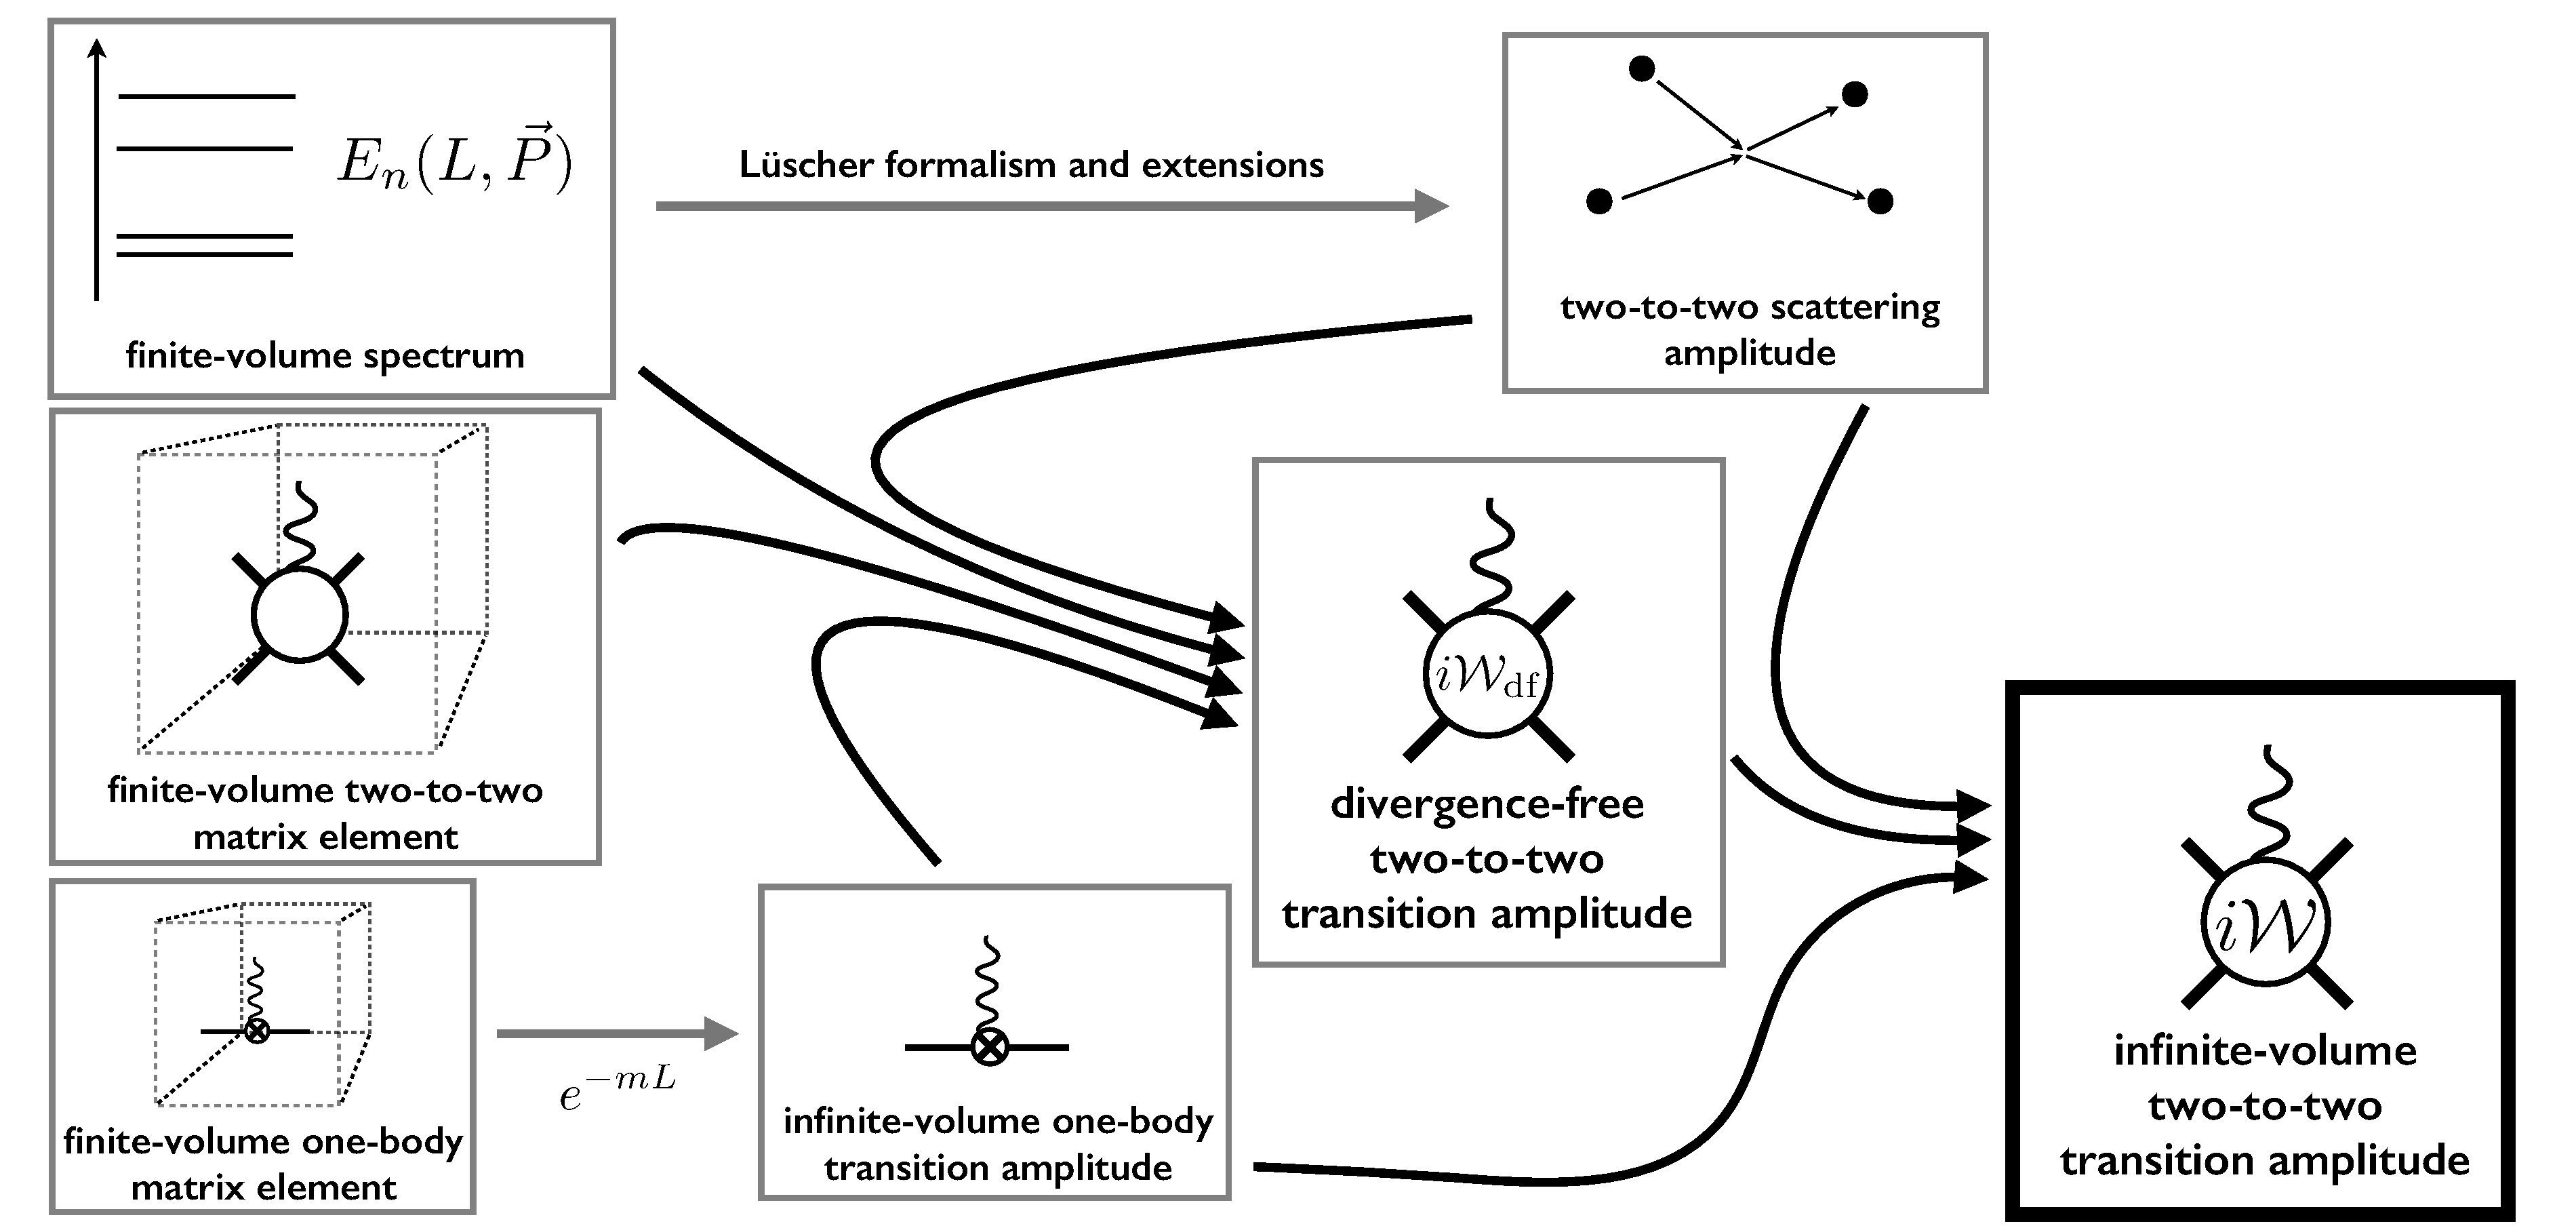
\includegraphics[width=.8\textwidth]{figs/flowchart2}}
\caption{Flowchart summarizing the process for extracting resonance form factors using the formalsim of Ref.~\cite{Briceno:2015tza}. {\mh [check update]}}\label{fig:flowchart}
\end{center}
\end{figure*}
 %%%%%%%%%%%%%%%%%%%%%%%%%%%%%%%%%%%%%%%%%%%

 %%%%%%%%%%%%%%%%%%%%%%%%%%%%%%%%%%%%%%%%%%
\subsection{Isospin and charge}

The aim of this project is to explain how one can obtain the form factors of a resonance. In particular, we will be focusing on electromagnetic form factors and to resonances that couple to $\pi\pi$ states. With this in mind, it is useful to review the isospin projections of the $\pi\pi$ system, and the resonance content of each channel, beginning with the isostensor. This channel has no resonances; the individual states are given by
\begin{align}
|I=2,m_I=2\rangle&=|\pi^+\pi^+\rangle \,,\\
|I=2,m_I=1\rangle&=\frac{1}{\sqrt{2}}\left(|\pi^+\pi^0\rangle+|\pi^0\pi^+\rangle\right) \,,\\
|I=2,m_I=0\rangle&=\frac{1}{\sqrt{6}}\left(|\pi^+\pi^-\rangle+|\pi^-\pi^+\rangle+2|\pi^0\pi^0\rangle\right) \,.
\end{align}

By contrast, the isovector channel contains the rho resonance, $\rho=(\rho^+,\rho^0,\rho^-)$. The $\rho^0$ is neutral and an eigenstate of charge conjugation. Furthermore, the electromagnetic current is odd under charge conjugation, $C\bar{\psi}\gamma^\mu \psi C=-\bar{\psi}\gamma^\mu \psi$. This implies 
\begin{align}
\langle \rho^0|\bar{\psi}\gamma^\mu \psi | \rho^0\rangle
=
\langle \rho^0|C(C\bar{\psi}\gamma^\mu \psi C)C| \rho^0\rangle
=
-\langle \rho^0|\bar{\psi}\gamma^\mu \psi | \rho^0\rangle=0.
\end{align}
Similarly, one concludes that the electromagnetic matrix elements of the $\pi^0$ vanishes. Note, since the $\rho^0$ is negative under charge conjugation and the $\pi^0$ is even, the $\langle \rho^0|\bar{\psi}\gamma^\mu \psi | \pi^0\rangle$ matrix element need not be zero, similarly the $\pi^0\to\gamma\gamma$ is not zero.

 Since the $\rho^0$ form factors are zero, we will focus on the $\rho^+$. The definition of $I=1$ $\pi\pi$ states and the association to the $\rho$ states is as follows:
\begin{align}
\rho^+:\hspace{.5cm}|I=1,m_I=1\rangle&=\frac{1}{\sqrt{2}}\left(|\pi^+\pi^0\rangle-|\pi^0\pi^+\rangle\right),\\
\rho^0:\hspace{.5cm}|I=1,m_I=0\rangle&=\frac{1}{\sqrt{2}}\left(|\pi^+\pi^-\rangle-|\pi^-\pi^+\rangle\right) \,.
\end{align}
Here we notice two things. As already stated above, we will need the form factors of the individual pions to calculate the rho form factor. Given that only that of the $\pi^+$ is nonzero, we will only need to calculate this one. 
 

Finally, the isoscalar channel couples to the $\sigma$,
\begin{align}
\sigma:\hspace{.5cm}|I=0,m_I=0\rangle&=\frac{1}{\sqrt{3}}\left(|\pi^+\pi^-\rangle+|\pi^-\pi^+\rangle-|\pi^0\pi^0\rangle\right).
\end{align}
This, of course, is neutral and is even under charge conjugation. As a result, similarly for the $\rho^0$ and $\pi^0$ its electromagnetic form factor vanishes. 

In conclusion, of the $\pi\pi$ channels, the one that is most sensible to consider here is $(I,m_I)=(1,1)$, since this is the only one that could have a resonance form factors. The $\rho^+$ is a vector, implying that it has three-independent form factors to determine, the charge, magnetic and quadrupole form factors. These are proportional to the the charge, magnetic moment, and quadrupole moment of the $\rho^+$. Furthermore, one can obtain the correspond radii of the $\rho^+$. As we argue below, in practice this \emph{might} require to calculate four independent amplitudes from lattice QCD calculations. As one analytically continues these onto the $\rho$ pole, one of them will vanish, resulting in three non-zero form factors. 


After examining which matrix elements are allowed in the following subsection, we discuss the Lorentz decomposition of the matrix elements in terms of form factors in Sec.~\ref{sec:Lorentz_FFs}.

 %%%%%%%%%%%%%%%%%%%%%%%%%%%%%%%%%%%%%%%%%%%%%%
 \subsection{Allowed matrix elements}

We are interested in evaluating matrix elements of the QED current
\begin{align}
{\mathcal{J}}^{\mu}=q_u\bar{u}\gamma^\mu u+q_d\bar{d}\gamma^\mu d= \big (2\bar{u}\gamma^\mu u-\bar{d}\gamma^\mu d \big )/3 \,.
\end{align} 
It is convenient to decompose this into an isovector and isoscalar current, 
\begin{align}
{\mathcal{J}}^{\mu}&=\frac{ \rho^{0,\mu}}{\sqrt{2}}+\frac{\omega^{\mu}}{3\sqrt{2}} \,,
\end{align}
where
\begin{align}
\rho^{0,\mu}&= \big ( \bar{u}\gamma^\mu u-\bar{d}\gamma^\mu d \big )/\sqrt{2} \,,\\
\omega^{\mu}&= \big (\bar{u}\gamma^\mu u+\bar{d}\gamma^\mu d \big )/\sqrt{2} \,.
\end{align} 
The $\rho^{0,\mu}$ component has the quantum number of the $I_z=0$ component of the $\rho$ meson, namely $I^G(J^{P})=1^{+}(1^{-})$,%
%FOOTNOTE
\footnote{$I=$isospin, $G=$G-parity, $J$=total angular momentum, $P$=parity.}
while the $\omega^{\mu}$ piece has the quantum numbers of the $\omega$ meson, $0^{-}(1^{-})$. Strictly speaking, these are the quantum numbers of the spatial piece of the current; the temporal components are related via Lorentz symmetry. 


For the single-pion matrix elements, one can explicitly evaluate the contractions {\raul (I get that the disconnected piece of the $\rho^{0,\mu}$ current vanishes, but not for the $\omega$ piece, so not $100\%$ sure about this)}, to find that only the component of the QED current that survives the $\rho$\,-like piece. {\mh [I am not so sure if it is true that we can see the vanishing by evaluating contractions. Consider in particular
\begin{align}
\langle \pi  \vert \omega^\mu \vert \pi \rangle & \propto \langle 0 \vert ( \bar q \tau^a \gamma_5 q )   (\bar{q} \mathbb I \gamma^\mu  q)  ( \overline q \tau^a \gamma_5 q  )\vert 0 \rangle \,, \\
& = - \text{Tr} \big [ S(i, f)  \tau^a \gamma_5  S(f,c) \mathbb I \gamma^\mu S(c,i) \tau^a \gamma_5 \big ] + \text{Tr} \big [ S(i, f)  \tau^a \gamma_5  S(f,i) \tau^a \gamma_5 \big ]  \text{Tr} \big [ S(c,c) \mathbb I \gamma^\mu  \big ] \,.
\end{align}
I don't there is an easy way to see that this is zero. One approach to argue that it vanishes is to note that a field configuration and its G-parity conjugate must have the same weight in the path integral. So one can consider the sum of these terms with their G-parity conjugates. I would suspect these should cancel to zero. But in the end this is the same as just studying the effect of G-parity on the matrix element and I think the latter is more elegant. So, if this is true, I would vote to drop discussion about contractions here. Of course it is still important to state that the disconnected part of the $\rho^{0,\mu}$ matrix element vanishes.]

}


\begin{align}
\langle\pi|{\mathcal{J}}^{\mu}|\pi\rangle=
\langle\pi|\rho^{0,\mu}|\pi\rangle/\sqrt{2}.
\end{align}

\bigskip

One can more generally find which components vanish, by considering the quantum numbers of the initial and final states in conjunction with those of the current. It is convenient to consider this in terms of a scattering process, $\pi\gamma^\star\to\pi$. The advantage of doing this is that one is explicitly reminded of the additional degrees of freedom associated with the the relative angular momentum ($\ell$) between the two initial particles. We also stress that this affects the total parity of the incoming state.


With this in mind, we tabulate all possible combinations of quantum numbers for $\pi\gamma^\star$ and check which configurations can overlap the final $\pi$
\begin{center}
\renewcommand{\arraystretch}{1.2}
 \begin{tabular}{ |c | c | c |c|c| c|} 
\hline 
\ \ current [$I^G(J^{P})$] \ \ 
& 
\ \ initial hadron \ \ 
&
\ \ relative $\ell$ \ \ 
&
\ \ possible final states \ \ 
& 
\ \ final hadron \ \ 
& 
\ \ overlap? \ \ 
%%%%%%%%%%%%%%%%%%%%%%%
\\ \hline \hline
\multirow{3}{*}{$\rho^{0,i}[1^{+}(1^{-})]$}
&
\multirow{3}{*}{$\pi[1^{-}(0^{-})]$}
&
$0$
&
$[1^{-}(1^{+})],\ldots$
&
\multirow{3}{*}{$\pi[1^{-}(0^{-})]$}
&No (violates $P$)
%%%%%%%%%%%%%%%%%%%%%%%
\\
&
&
$1$
&
$[1^{-}(0^{-})],[1^{-}(1^{-})],\ldots$
&
& Yes 
%%%%%%%%%%%%%%%%%%%%%%%
\\
&
&
$\geq 2$
&
$ [1^- (J \geq 1)], \dots $
&
& No (violates $J$) 
%%%%%%%%%%%%%%%%%%%%%%%
\\\hline \hline
$\omega^{i}[0^{-}(1^{-})]$
&
$\pi[1^{-}(0^{-})]$
& $\geq 0$
& $[1^+ (J \geq 0)]$
&
$\pi[1^{-}(0^{-})]$
& No (violates $G$)
%%%%%%%%%%%%%%%%%%%%%%%
\\ \hline
\end{tabular}
 \end{center}
{\mh (We conclude the same result found by studying contractions above, that only one component of the current contributes to this transition.)} The ellipsis in the first two lines denotes other components of isospin that do not contribute. 

 \bigskip

Now, we turn to the target $\pi\pi\gamma^\star\to\pi\pi$ transitions. As already discussed above, we focus attention on the scenario where the $\pi\pi$ state has been projected onto the quantum numbers of the $\rho$. Therefore, we can equally well tabulate the allowed quantum numbers for $\rho\gamma^\star\to\rho$, 
\begin{center}
\renewcommand{\arraystretch}{1.2}
 \begin{tabular}{ |c | c | c |c|c| c|} 
\hline 
\ \ current [$I^G(J^{P})$] \ \ 
& 
\ \ initial hadron \ \ 
&
\ \ relative $\ell$ \ \ 
&
\ \ possible final states \ \ 
& 
\ \ final hadron \ \ 
& 
\ \ overlap? \ \ 
%%%%%%%%%%%%%%%%%%%%%%%
\\\hline \hline
\multirow{5}{*}{$\rho^{0,i}[1^{+}(1^{-})]$}
&
\multirow{5}{*}{$\rho^{0,i}[1^{+}(1^{-})]$}
&
0
&
$[1^{+}(1^{+})],\ldots$
&
\multirow{5}{*}{$\rho^{0,i}[1^{+}(1^{-})]$}
&No (violates $P$)
%%%%%%%%%%%%%%%%%%%%%%%
\\
&
&
1
&
$[1^{+}(0^{-})],[1^{+}(1^{-})],\ldots$
&
& Yes
%%%%%%%%%%%%%%%%%%%%%%%
\\
&
&
2
&
$[1^{+}(0^{+})],[1^{+}(1^{+})],\ldots$
&
& No (violates $P$)
%%%%%%%%%%%%%%%%%%%%%%%
\\
&
&
3
&
$[1^{+}(1^{-})],\ldots$
&
& Yes
%%%%%%%%%%%%%%%%%%%%%%%
\\
&
&
$\geq 4$
&
$[1^{+}(J \geq 2)], \ldots$
&
& No (violates $J$)
%%%%%%%%%%%%%%%%%%%%%%%
\\\hline \hline
$\omega^{i}[0^{-}(1^{-})]$
&
$\rho^{0,i}[1^{+}(1^{-})]$
& $ \geq 0$
& $[1^- (J \geq 0)]$
&
$\rho^{0,i}[1^{+}(1^{-})]$
&No (violates $G$) 
  \\ \hline
\end{tabular}
 \end{center}
Again, we get that this transition is allowed and only the $\rho$ component of the current contributes. {\mh In a nut shell, because $\omega$ flips $G$-parity it can only mediate transitions where the initial- and final-state G-parity differ.}

{\mh [Please check changes to both tables]}

{\mh [Question: We know with parity that, in addition to the intrinsic part, we must keep track of the parity induced by the $\ell$ value. Are we sure that nothing like this happens with $G$? For example it could be that the total $G$ parity is not just the product of intrinsic parities but also some contribution that depends on the total isospin of the final state. Just wanna be sure we are not missing something...]}

\bigskip

{\mh In summary, the following matrix elements are allowed
\begin{gather}
\overline F_{J=0}(p_f, p_i) \equiv \big  \langle \pi [1^- (0^-)] \big \vert \Big [ \rho^{0,\mu}  \big \vert \pi [1^- (0^-)] \big \rangle \Big ]_{[\ell=1,\ 1^- (0^-)]}   \,, \\
  \big  \langle \rho^{0,i} [1^+ (1^-)] \big \vert \Big [ \rho^{0,\mu}  \big\vert \rho^{0,i} [1^+ (1^-)]  \big\rangle \Big ]_{[\ell=1,\ 1^+ (1^-)]}   \,, \\
  \big  \langle \rho^{0,i} [1^+ (1^-)] \big \vert \Big [ \rho^{0,\mu} \big \vert \rho^{0,i} [1^+ (1^-)] \big \rangle \Big ]_{[\ell=3,\ 1^+ (1^-)]}   \,.
\end{gather}

The meaning of these is relatively obscure, consider for example $\overline F_{J=0}(p_f, p_i)$. To define this we first introduce
\begin{equation}
F^\mu(p_f, p_i)  \equiv \langle \pi(p_f) \vert \rho^{0, \mu}(0) \vert \pi (p_i) \rangle \,.
\end{equation}
Then, introducing ${\Lambda^\mu}_\nu$ as the boost to the $\textbf p_f=0$ frame we define
\begin{equation}
\overline F^\mu(\bar p_f^0, \bar p_i^0, \bar {\textbf p}_i)  \equiv {\Lambda^\mu}_\nu  F^\nu(p_f, p_i)  \,,
\end{equation}
where $\bar p^\mu \equiv {\Lambda^\mu}_\nu p^\nu$. Note that in defining $\overline F$ we have done two things (1) boosted the original $F^\mu$ to the $\textbf p_f=0$ frame and (2) rexpressed the quantity as a function of momenta defined in that frame.

We are now in position to define the projection to definite $\lambda$ and to definite $m$ with $\ell=1$
\begin{equation}
\overline F_{m; \lambda}(\bar p_f^0, \bar p_i^0, \vert \bar {\textbf p}_i\vert) \equiv A \, \epsilon_\mu(\bar p_f - \bar p_i, \lambda) \int d \Omega_{\hat {\textbf p}_i} Y_{1 m}(\hat {\textbf p}_i) \overline F^\mu(\bar p_f^0, \bar p_i^0, \bar {\textbf p}_i)  \,,
\end{equation}
and to combine to $J=0$
\begin{equation}
\overline F_{J=0}(\bar p_f^0, \bar p_i^0, \vert \bar {\textbf p}_i\vert)  = \sum_{m,\lambda} C^{J=0,m_J=0}_{1 m; 1 \lambda} \overline F_{m; \lambda}(\bar p_f^0, \bar p_i^0, \vert \bar {\textbf p}_i\vert)  \,.
\end{equation}
Here $A$ is a numerical prefactor to be chosen for convenience.

[At this point it is not clear whether it is really necessary to perform these projections. Perhaps thinking of the $\pi \gamma^*$ state is just a useful trick for deciding which matrix elements are allowed. Once we know these there is no need to project to them explicitly.]


}


 \subsection{Lorentz decomposition in terms of form factors \label{sec:Lorentz_FFs}}
When considering QCD stable states, it is naturally to write the matrix elements of the QED current in terms of form factors up to overall factors which are completely constraints from kinematics. Here, we review this for matrix elements coupling pseudoscalar and vectors states. In this study, we are primarily interested on currents coupling to the $\pi$ and $\rho$. In this section, we will ignore the fact that the $\rho$ is unstable, and we address this in Sec.~\ref{sec:Lorentz_amps}. Furthermore, for the sake of generality, when considering matrix elements coupling pseudoscalar-to-pseudoscalar states or vector-to-vector states, we will not assume that the initial and final states are degenerate. As we will see below, this is essential for later addressing the unstable nature of the $\rho$. To accommodate this added complexity, we will introduce another species of pseusocalar and vector mesons, which will refer to as $\pi'$ and $\rho'$ respectively, which will also be assumed to be stable in this section. 



\subsubsection{Lorentz decomposition of $\pi\gamma^\star\to\pi'$}
We begin with the elastic pion matrix elements, $\langle\pi(p_f)|{\mathcal{J}}^{\mu}|\pi(p_i)\rangle$. This matrix element is a Lorentz vector, therefore it can only be proportional to linear combinations of the two vectors in the problem ($p_i^\mu, p_f^\mu$),
\begin{align}
\langle\pi(p_f)|{\mathcal{J}}^{\mu}|\pi(p_i)\rangle=F_\pi(Q^2)\,(p_i+p_f)^\mu+F_{\pi,-}(Q^2)\,(p_i-p_f)^\mu,
\end{align}
where $F_\pi(Q^2)$ and $F_{\pi,-}(Q^2)$ are unknown form factors that in general depend on any Lorentz scalar in the system: $Q^2=(p_i-p_f)^2, p_i^2=m_\pi^2,$ and $p_f^2=m_\pi^2$. Here, we leave the dependence on the pion mass implicit. 

The current ${\mathcal{J}}^{\mu}$ is conserved, $\partial_\mu {\mathcal{J}}^{\mu}=0$, which in momentum space tells us that 
\begin{align}
(p_i-p_f)_\mu\langle\pi(p_f)|{\mathcal{J}}^{\mu}|\pi(p_i)\rangle&=F_\pi(Q^2)\, (p_i-p_f)_\mu(p_i+p_f)^\mu+F_{\pi,-}(Q^2)\,(p_i-p_f)^2
\nn\\
&=
F_\pi(Q^2)\, (m_\pi^2-m_\pi^2)
+
F_{\pi,-}(Q^2)\,(p_i-p_f)^2
=0,
\end{align}
we conclude that $F_{\pi,-}(Q^2)$ must be zero for all virtualities. This is why for the pion we only need to determine a single form factor. 

Note, in the last line above, the first term vanished because the initial and final states have the same mass. If we consider two pseudoscalars with different masses, the $\pi$ and $\pi'$, then charge conservation would lead to
\begin{align}
(p_i-p_f)_\mu\langle\pi(p_f)|{\mathcal{J}}^{\mu}|\pi'(p_i)\rangle&=
F_{\pi\pi'}(Q^2)\, (m_{\pi'}^2-m_\pi^2)
+
F_{\pi\pi',-}(Q^2)\,(p_i-p_f)^2
=0,
\\
\Rightarrow
F_{\pi\pi',-}(Q^2)
&=-
F_{\pi\pi}(Q^2)\, \frac{(m_{\pi'}^2-m_\pi^2)}{(p_i-p_f)^2}
= 
F_{\pi\pi}(Q^2)\, \frac{(m_{\pi'}^2-m_\pi^2)}{Q^2}.
\end{align} 
In this case we conclude that one can still describe this matrix element using is a single form factor
\begin{align}
\langle\pi(p_f)|{\mathcal{J}}^{\mu}|\pi'(p_i)\rangle=
\left( (p_i+p_f)^\mu \, +(p_i-p_f)^\mu\frac{(m_{\pi'}^2-m_\pi^2)}{Q^2}\right)F_{\pi\pi}(Q^2).
\label{eq:pi_to_pi_FF}
\end{align}
Again, $F_{\pi\pi}(Q^2)$ depends on the masses of the two states. {\mh  Hermiticity, together with time-reversal invariance, ensures that it must be symmetric on the interchange of these two
\begin{equation}
F_{\pi\pi}(m^2_\pi, m'^2 _\pi,Q^2) = F_{\pi\pi}(m'^2_\pi, m^2 _\pi,Q^2) \,.
\end{equation}}
Below we consider examples when the decomposition is less trivial.  



\subsubsection{Lorentz decomposition of $\rho\gamma^\star\to\pi$}

Now, we turn to a slightly more complicated case, where a stable vector meson couples to a pseudoscalar.  In this case, the matrix element must be Lorentz vector. This is a bit difficult to see, since states in flight are not eigenstates of parity. This further complicated by the fact that the $\rho$ has nonzero spin~\cite{Thomas:2011rh}. Nevertheless, we can derive the form of the Lorentz decomposition of the matrix element in a relatively straightforward manner.

First, the $\rho$ state is now defined by its momentum and helicity, $\lambda$. In the limit that the momentum is taken to be zero, we choose to quantize the spin along the $z$ axis.  Next, we note that the matrix element we are after, must be proportional to the polarization of the polarization vector of the $\rho$,
\begin{align}
\langle \pi(p_f)|\mathcal{J}^\mu|\rho(\lambda; p_i)\rangle\propto \epsilon^\nu(\lambda; p_i),
\end{align}
note the Lorentz index of $\epsilon^\nu$ need not coincide with that of the current. 

There are only three linearly independent components of a spin-1 vector meson. This is manifested by the fact that $\epsilon_{\mu}(\lambda, p)p^{\mu}=0$. A standard choice for the polarization vectors that is normalized to $-1$ and satisfies this criterion is{ \begin{align}
\epsilon^{\mu}(\lambda, p) & =
\left(\frac{\vec{p}\cdot\hat{e}_\lambda}{ \sqrt{p^2} }, \ \hat{e}_\lambda + \frac{1}{\vec p^{\,2}} \left( \frac{p^0}{\sqrt{p^2}} - 1  \right) {\vec{p}\cdot\hat{e}_\lambda} \ \vec{p}\right) 
.
%  =  \left(\frac{\vec{p}\cdot\hat{e}_\lambda}{ \sqrt{p^2} }, \ \hat{e}_\lambda +   \frac{\vec{p}\cdot\hat{e}_\lambda  }{\sqrt{p^2} \left( \sqrt{p^2} + p^0 \right) }    \vec{p}\right) \,.
\end{align}
This satisfies the orthogonality via
 \begin{align}
\epsilon^{\mu}(\lambda, p) p_\mu = p^0 \frac{\vec{p}\cdot\hat{e}_\lambda}{\sqrt{p^2} }  -  \hat{e}_\lambda \cdot \vec p - \left( \frac{p^0}{\sqrt{p^2}} - 1  \right) \vec{p}\cdot\hat{e}_\lambda   = 0 \,,
\end{align}
and normalization via
\begin{align}
\epsilon^{\mu}(\lambda, p) \epsilon_{\mu}(\lambda, p) & = \frac{\vec p^{\,2}}{p^2}  ( \hat{p}\cdot\hat{e}_\lambda)^2 - \left [  \hat{e}_\lambda +   \left( \frac{p^0}{\sqrt{p^2}} - 1  \right) { {\hat p}\cdot\hat{e}_\lambda} \  {\hat p}\right] ^2  \\
& = \frac{\vec p^{\,2}}{p^2} ( \hat{p}\cdot\hat{e}_\lambda)^2 - 1 -    \left( \frac{p^0}{\sqrt{p^2}} - 1  \right)^2 ( { {\hat p}\cdot\hat{e}_\lambda} )^2    - 2    \left( \frac{p^0}{\sqrt{p^2}} - 1  \right) ({ {\hat p}\cdot\hat{e}_\lambda}  )^2 \,, \\
& = -1 + ( \hat{p}\cdot\hat{e}_\lambda)^2 \left[ \frac{\vec p^{\,2}}{p^2}  - \frac{(p^0)^2}{p^2} - 1 + 2 \frac{p^0}{\sqrt{p^2}}     - 2    \frac{p^0}{\sqrt{p^2}} + 2      \right ] \,, \\
& = -1 \,.
\end{align}

Here we use the four-dimensional units vectors
\begin{align}
\hat{e}_\pm&=\mp\frac{1}{\sqrt{2}}(0,1,\pm i,0),
\\
\hat{e}_0&=(0,0,0,1).
\end{align}
It is important to note that $\epsilon^\mu(p,\lambda)$ is a pseudovector. 

Under parity transformations, $\hat{P}$, the momentum of a state changes direction but its spin remains unchanged. Given that helicity is defined as the component of the spin along the direction of the momentum, under parity transformations the helicity changes sign. For example, the $\rho$ state would transform as
\begin{align}
\hat{P}|\rho(\lambda, p_i)\rangle
=-|\rho(-\lambda, (p_{i,0},-\vec{p}_i)\rangle,
\end{align}
where the overall phase is due to the $\rho$ intrinsic negative parity. If instead the $\rho$ is at rest, defined by $p_i=(m_\rho,\vec{0})$, and denote the azimuthal component of its spin as $m_z$, then
\begin{align}
\hat{P}|\rho(m_z, (m_\rho,\vec{0}))\rangle
=-|\rho(m_z, (m_\rho,\vec{0})\rangle,
\end{align}
and the $\rho$ would indeed be an eigenstate of parity. 

With this in mind, let us consider the matrix element in the frame where the $\rho$ is at rest. Under parity, this would transform as
\begin{align}
\langle \pi(p_f)|\mathcal{J}^\mu|\rho(\lambda; p_i)\rangle
=
\langle \pi(p_f)|\hat{P}\hat{P}\mathcal{J}^\mu\hat{P}\hat{P}|\rho(\lambda, p_i)\rangle
=
(-1)^2\langle \pi(p_f^0,-\vec{p}_f)|\mathcal{J}_\mu|\rho(\lambda, p_i)\rangle
=\langle \pi(p_f^0,-\vec{p}_f)|\mathcal{J}_\mu|\rho(\lambda, p_i)\rangle.
\end{align}
Immediately, we see that the Lorentz structure of the matrix does not coincide with that of the polarization vector. The only other two vector we have at our disposal are $p_i$ and $p_f$. Requiring the matrix element to be proportional to the polarization vector, we find that the only allowed Lorentz structure is the following
\begin{align}
\langle \pi(p_f)|\mathcal{J}^\mu|\rho(\lambda, p_i)\rangle
=
\epsilon^{\mu\alpha\beta\gamma}p_{f,\alpha}p_{i,\beta}\epsilon_\gamma F_1(Q^2,p_i^2,p_f^2)
\label{eq:pi_to_rho_FF}
\end{align}
note, a term of the form $p^\mu_{f}\,(p_{i}\cdot\epsilon)$ is exactly equal to zero. We also can rule out a term of the form $p^\mu_{i}\,(p_{f}\cdot\epsilon)$ because in the rest frame of the $\rho$, under parity this would trasnform as 
\begin{align}
p^\mu_{i}\,(p_{f}\cdot\epsilon) 
=(-m_\rho \,\vec{p}_{f}\cdot\vec{\epsilon},\vec{0})
\to (m_\rho \,\vec{p}_{f}\cdot\vec{\epsilon},\vec{0}).
\end{align}
Similarly, we can rule out a term of the form $p^\mu_{i}\,(p_{i}\cdot\epsilon)$. {\raul Note, Hemiticity also rules out terms proportional to $p^\mu_{i}\,(p_{f}\cdot\epsilon)$ or $p^\mu_{f}\,(p_{f}\cdot\epsilon)$. [need to think of this more...]}

\subsubsection{Lorentz decomposition of $\rho\gamma^\star\to\rho'$}

Now, we turn to the case where we have a stable spin-1 particle in the initial and final state. Once again, the matrix element must be proportional to the polarization vector of the initial state, $\epsilon^{\mu}(\lambda_i, p_i)$, and conjugate polarization vector of the final state, $\epsilon^{* \mu}(\lambda_f,p_f)$.  To systematically ensure that all possible structures are included, we first list all possible building blocks that carry a Lorentz index:
\begin{gather}
p_f^\mu,\ p_i^\mu,\ \epsilon^{*\mu}_f,\ \epsilon_i^{\mu} \,.
\end{gather}
Since the matrix element must be proportional to both polarization vectors, the following decomposition must hold:
\begin{multline}
\langle\rho'(\lambda_f,p_f)|{\mathcal{J}}^{\mu}|\rho(\lambda_i,p_i)\rangle
=
\big ( \epsilon_f^*\cdot \epsilon_i \big ) \  {X}^\mu \big (p_i^\alpha,p_f^\beta \big)
+ \epsilon_i^\mu    \Big ( \epsilon_f^* \cdot {Y_f} \big (p_i^\alpha,p_f^\beta \big) \Big ) 
+ \epsilon_f^{*\mu}  \Big (  \epsilon_i \cdot {Y_i}  \big (p_i^\alpha,p_f^\beta \big)  \Big ) \\ 
+  \epsilon_f^{*\nu}   \epsilon_i^\sigma {Z^{\mu}}_{\nu \sigma}  \big (p_i^\alpha,p_f^\beta \big) \,.
\end{multline}
 
 Here we have separated out all ways in which the indices on the polarization vectors can enter the vector matrix element. The key point is that $X$, $Y_i$, $Y_f$ and $Z$ are tensors, transforming as indicated by the the index structure, that do not depend on the polarization. In particular, the decomposition of $X^\mu$, $Y_i^\mu$, $Y_f^\mu$, must be identical to that of the pion vector matrix element, i.e.
\begin{equation}
{X}^\mu \big (p_i^\alpha,p_f^\beta \big) = (p_i + p_f)^\mu X_+ \big (Q^2, p_i^2,p_f^2 \big) + (p_i - p_f)^\mu {X_-} \big (Q^2, p_i^2,p_f^2 \big) \,.
\end{equation}
By contrast, the three-index quantity $Z^{\mu \nu \sigma}$ leads to a new decomposition
\begin{multline}
Z^{\mu \nu \sigma} \big (p_i^\alpha,p_f^\beta \big) = \sum_{a,b,c=i,f} p_a^\mu p_b^\nu p_c^\sigma Z_{abc} \big (Q^2, p_i^2,p_f^2 \big) \\ 
+ g^{\mu \nu}  Z^\sigma_i \big (Q^2, p_i^2,p_f^2 \big) + g^{\mu \sigma}  Z^\nu_f \big (Q^2, p_i^2,p_f^2 \big) + g^{\nu \sigma}  Z^\mu \big (Q^2, p_i^2,p_f^2 \big) \,.
\end{multline}
{\raul [Since $Z^\sigma_i  $ is a vector, shouldn't it depend on the two vectors in the problem $p_i^\alpha,p_f^\beta$ instead of just the scalars? ]} 

{\mh
Further decomposing the one-index $Z$ functions on the second line leads to a total of $14$ scalar form factors for the three-index quantity. However the second line leads only to terms redundant with those from $X$, $Y_i$ and $Y_f$. Dropping these leads to $8$ remaining terms from $Z$. These are to be combined with $2$ each from $X$, $Y_i$ and $Y_f$ for a grand total of $14$. Of these $14$, $8$ are redundant due to the identity $p_i\cdot \epsilon_i=p_f\cdot \epsilon_f^*=0$. More specifically, $X$ generates 2 distinct contributions, $Y_i$ and $Y_f$ each give 1, and in the end $Z$ only generates 2 more. } 

{\raul [I find this discussion slightly complicated and a bit circular. In particular, the fact that we introduce new terms written in a different way but then say that they are the same as the ones we already wrote down. An alternative starting point that is slightly less redundant is 
\begin{multline}
\langle\rho'(\lambda_f,p_f)|{\mathcal{J}}^{\mu}|\rho(\lambda_i,p_i)\rangle
=
\big ( \epsilon_f^*\cdot \epsilon_i \big ) \  {X}^\mu \big (p_i^\alpha,p_f^\beta \big)
+ \epsilon_i^\mu    \Big ( \epsilon_f^* \cdot {Y_f} \big (p_i^\alpha,p_f^\beta \big) \Big ) 
+ \epsilon_f^{*\mu}  \Big (  \epsilon_i \cdot {Y_i}  \big (p_i^\alpha,p_f^\beta \big)  \Big ) \\ 
+  \epsilon_f^{*\nu}   \epsilon_i^\sigma 
\sum_{a,b,c=i,f} p_a^\mu p_b^\nu p_c^\sigma Z_{abc} \big (Q^2, p_i^2,p_f^2 \big)
 \,.
\end{multline}
This also avoids introducing $Z$ functions that are then written in terms of other $Z$ functions.
]}



We deduce that Lorentz invariance alone restricts the decomposition to $6$ distinct, nonzero scalar form factors. After slight rearanging these can be written
\begin{equation}
\begin{split}
\langle\rho'(\lambda_f,p_f)|{\mathcal{J}}^{\mu}|\rho(\lambda_i,p_i)\rangle
&=
(p_f+p_i)^\mu \,\epsilon_f^*\cdot \epsilon_i\, \widetilde{G}_1(Q^2,p_i^2,p_f^2)
\\&
+(p_i-p_f)^\mu \,\epsilon_f^*\cdot \epsilon_i\,\widetilde{G}_2(Q^2,p_i^2,p_f^2)
\\&
+\left(\epsilon_i^\mu\, p_i\cdot \epsilon_f^*\,+\epsilon_f^{*\mu}\, p_f\cdot \epsilon_i\right)
\,\widetilde{G}_3(Q^2,p_i^2,p_f^2)
\\&
+\left(\epsilon_i^\mu\, p_i\cdot \epsilon_f^*\,-\epsilon_f^{*\mu}\, p_f\cdot \epsilon_i\right)
\,\widetilde{G}_4(Q^2,p_i^2,p_f^2)
\\&
+(p_f+p_i)^\mu \,(\epsilon_f^*\cdot p_i)\,(\epsilon_i\cdot p_f)\,\widetilde{G}_5(Q^2,p_i^2,p_f^2)
\\&
+(p_i-p_f)^\mu \,(\epsilon_f^*\cdot p_i)\,(\epsilon_i\cdot p_f)\,\widetilde{G}_6(Q^2,p_i^2,p_f^2).
\end{split}
\end{equation}
% In total we find six possible structures, where we excluded terms of the form $p_i\cdot \epsilon_i=p_f\cdot \epsilon_f^*=0$.

 Next we show that time-reversal invariance implies that all six scalar form factors are real functions of $Q^2,p_i^2,p_f^2$. We begin by
considering a specific interpolator for the rho
\begin{equation}
\vert \rho^+( \lambda_{\textbf{p}}, \textbf p ) \rangle =  \lim_{p^0 \to \omega_\textbf p}  \epsilon_{\mu}(\lambda_{\textbf{p}}, p)(1/i) [- (p^0)^2 + \textbf p^2 + m^2] \int d^4 x e^{- i p^0  x^0 + i \textbf p \cdot \textbf x} \ \overline d(x) \gamma^\mu u(x) \vert 0 \rangle \,,
\end{equation}
where we introduced an index in the helicity to denote witch which axis it is defined. Note $\lambda_{\textbf{p}}=(-1)^{\lambda_{\textbf{p}}}\lambda_{\textbf{-p}}$. Acting with the time-reversal operator on this state gives
\begin{equation}
T \vert \rho^+( \lambda_{\textbf{p}}, \textbf p) \rangle =  \lim_{p^0 \to \omega_\textbf p} \epsilon^*_{\mu}(\lambda_{\textbf{p}}, p) i [- (p^0)^2 + \textbf p^2 + m^2] \int d^4 x e^{ i p^0  x^0 - i \textbf p \cdot \textbf x} \ T \overline d(x) \gamma^\mu u(x)     T^{-1} \  \vert 0 \rangle \,.
\end{equation}
To simplify this we substitute $\epsilon^{\mu*}( \lambda_{\textbf{p}}, p) = (-1)^\lambda \epsilon^{\mu}( - \lambda_{\textbf{p}} , p)$ and%
%
\footnote{
The identify for $\epsilon^{\mu*}( p, \lambda) $ follows from the definition
\begin{align}
\epsilon^{\mu}(p,\lambda) & =
\left(\frac{\vec{p}\cdot\hat{e}_\lambda}{ \sqrt{p^2} }, \ \hat{e}_\lambda + \frac{1}{\vec p^{\,2}} \left( \frac{p^0}{\sqrt{p^2}} - 1  \right) {\vec{p}\cdot\hat{e}_\lambda} \ \vec{p}\right) \,,
\end{align} 
together with $\hat{e}_{\lambda}^* = (-1)^\lambda \hat{e}_{-\lambda}$.
}
%  
\begin{equation}
T \overline d(x) \gamma^\mu u(x)     T^{-1} = - {\mathcal T^\mu}_\nu \overline d(\mathcal T x) \gamma^\nu u(\mathcal T x)     \,,
\end{equation}
to reach
\begin{align}
T \vert \rho^+( \lambda_{\textbf{p}}, \textbf p) \rangle & =   (- 1)^{\lambda_{\textbf{p}}}  \  \lim_{p^0 \to \omega_\textbf p}   {\mathcal T^\mu}_\nu   \epsilon_{\mu}(- \lambda_{\textbf{p}}, p) (1/i) [- (p^0)^2 + \textbf p^2 + m^2] \int d^4 x e^{ i p_\mu {\mathcal T^\mu}_\nu  x^\nu} \   \overline d(x) \gamma^\nu u(x)      \vert 0 \rangle \,, 
\end{align}
Finally using $ {\mathcal T^\mu}_\nu \epsilon_{\mu}(p, - \lambda_{\textbf{p}}) = \epsilon_{\nu}(p^0, - \textbf p, - \lambda_{\textbf{p}})$, we conclude
\begin{equation}
 T \vert \rho^+(\lambda_{\textbf{p}}, \textbf p) \rangle = (-1)^{\lambda_{\textbf{p}}} \vert \rho^+(- \lambda_{\textbf{p}} ,- \textbf p) \rangle
 = (-1)^{\lambda_{\textbf{p}}} \vert \rho^+( \lambda_{-\textbf{p}} ,- \textbf p) \rangle \,.
\end{equation}
Note, the spin and momentum change sign, as expected, which implies that that the helicity does not flip sign. 

Next we use the identity
\begin{equation}
  \langle \alpha \vert  \mathcal O \vert \beta \rangle    =  \left [ \Big ( T \vert \alpha \rangle \Big )^\dagger   T \mathcal O T^{-1}  \Big ( T \vert \beta \rangle \Big ) \right ]^* \,,
\end{equation}
to write
\begin{equation}
\langle\rho'(\lambda_f,p_f)|{\mathcal{J}}^{\mu}|\rho(\lambda_i,p_i)\rangle =- (-1)^{\lambda_i+\lambda_f}  \mathcal {T^{\mu}}_\nu \langle\rho'(- \lambda_f, - \textbf p_f)|{\mathcal{J}}^{\nu}|\rho(- \lambda_i, - \textbf p_i)\rangle^*  \,.
\end{equation}
{\raul [Not sure I understand this equation. Using what we found above, we have
\begin{align}
 T T \vert \rho^+(\lambda_{\textbf{p}}, \textbf p) \rangle = (-1)^{\lambda_{\textbf{p}}}T \vert \rho^+(- \lambda_{\textbf{p}} ,- \textbf p) \rangle
 =
(-1)^{\lambda_{\textbf{p}}-\lambda_{\textbf{p}}} \vert \rho^+( \lambda_{\textbf{p}} , \textbf p) \rangle
= 
\vert \rho^+( \lambda_{\textbf{p}} , \textbf p) \rangle
\end{align}
meaning $T^2=1$ and $T=T^{-1}$. So then 
\begin{align}
  \langle \rho^+(\lambda_{\textbf{p}'}, \textbf p') \vert  \mathcal \mathcal{J}^{\mu} \vert \rho^+(\lambda_{\textbf{p}}, \textbf p) \rangle   
  & = 
  \langle \rho^+(\lambda_{\textbf{p}'}, \textbf p') \vert  T^2\mathcal \mathcal{J}^{\mu} T^2\vert \rho^+(\lambda_{\textbf{p}}, \textbf p) \rangle 
 \nn\\&
 =
 (-1)^{\lambda_{\textbf{p}}+\lambda_{\textbf{p}'}}
  \langle \rho^+(-\lambda_{\textbf{p}'}, -\textbf p') \vert  \mathcal \mathcal{J}_{\mu} \vert \rho^+(-\lambda_{\textbf{p}}, -\textbf p) \rangle 
 \nn\\&
 = 
  (-1)^{\lambda_{\textbf{p}}+\lambda_{\textbf{p}'}}
\bigg(\langle \rho^+(-\lambda_{\textbf{p}}, -\textbf p) \vert  \mathcal \mathcal{J}^*_{\mu} \vert \rho^+(-\lambda_{\textbf{p}'}, -\textbf p') \rangle \bigg)^*
 \nn\\
 &=
  (-1)^{\lambda_{\textbf{p}}+\lambda_{\textbf{p}'}}
 \bigg(\langle \rho^+(-\lambda_{\textbf{p}}, -\textbf p) \vert  \mathcal \mathcal{J}_{\mu} \vert \rho^+(-\lambda_{\textbf{p}'}, -\textbf p') \rangle \bigg)^*
\end{align}
where in going from the third to fourth equality I used the fact that the current is Hermitian.
]
}

To understand the consequences of this identity, suppose that only the first form factor, $\widetilde G_1$ were nonzero. This would imply
\begin{align}
(p_f+p_i)^\mu \,\epsilon_f^*  \cdot \epsilon_i \, \widetilde{G}_1(Q^2,p_i^2,p_f^2) & = \Big [ - (-1)^{\lambda_i+\lambda_f}  \mathcal {T^{\mu}}_\nu  \mathcal {P^{\nu}}_\alpha  (p_f+p_i)^\alpha \,\epsilon^*(- \lambda_f,  p_f) \cdot \epsilon(- \lambda_i,   p_i) \, \widetilde{G}_1(Q^2,p_i^2,p_f^2) \Big ]^* \,, \\
& =  \Big [ -    \mathcal {T^{\mu}}_\nu  \mathcal {P^{\nu}}_\alpha  (p_f+p_i)^\alpha \,\epsilon_f \cdot \epsilon^*_i \, \widetilde{G}_1(Q^2,p_i^2,p_f^2) \Big ]^* \,, \\
& =     (p_f+p_i)^\mu \,\epsilon^*_f \cdot \epsilon_i \, \widetilde{G}^*_1(Q^2,p_i^2,p_f^2)  \,,
\end{align}
where in the first line we used $\epsilon^*(- \lambda_f,  (p^0_f, - \textbf p_f)) \cdot \epsilon(- \lambda_i,   (p^0_f, - \textbf p_i)) = \epsilon^*(- \lambda_f,  p_f) \cdot \epsilon(- \lambda_i,   p_i)$. We deduce
\begin{equation}
\widetilde{G}_1(Q^2,p_i^2,p_f^2)  = \widetilde{G}^*_1(Q^2,p_i^2,p_f^2) \,.
\end{equation}
A similar argument can be used to show that all six scalar form factors satisfy this condition. [Check this!]

\bigskip
}




{\mh 
We next turn to the parity invariance of the theory. Note that, while $\epsilon_f^{*\mu}$ is a pseudovector, the product $\big ( p_f\cdot {\epsilon}_i \big ) \, \epsilon_f^{*\mu}$ defines a regular (non-pseudo) vector. This is because the combination $ p_f\cdot \epsilon_i$ is a pseudoscalar. %  It is worth remarking about the presence of the terms of the form $\epsilon_f^{*\mu}\, p_f\cdot \epsilon_i$. Naively, one might guess that these transform as pseudovectors, but if we pick the rest frame of the initial state, we find that under parity this transforms as 
In particular
\begin{equation}
\big ( p_f\cdot {\epsilon}_i \big ) \, \epsilon_f^{*\mu} \underset{P}{\longrightarrow} \big ( \! - p_f\cdot {\epsilon}_i \big ) \, \Big [ \! - {\mathcal P^\mu}_\nu \epsilon_f^{*\nu} \Big ] = {\mathcal P^\mu}_\nu \, \big ( p_f\cdot {\epsilon}_i \big ) \, \epsilon_f^{*\nu}   \,.
\end{equation}}
{\raul \begin{align}
\epsilon_f^{*\mu}\, p_f\cdot \vec{\epsilon}_i
&=
-\epsilon_f^{*\mu}\, \vec{p}_f \cdot\vec{\epsilon}_i\nn\\
&=
\left(\frac{\vec{p}_f\cdot\hat{e}_{\lambda_f}}{\sqrt{p^2_f}},\hat{e}_{\lambda_f}+\frac{\vec{p}_f\cdot\hat{e}_{\lambda_f}}{\sqrt{p^2_f}\left(\sqrt{p^2_f}+p^0_f\right)}\vec{p}_f\right)
\vec{p}_f \cdot\vec{\epsilon}_i
\nn\\
&\to
-
\left(-\frac{\vec{p}_f\cdot\hat{e}_{-\lambda_f}}{\sqrt{p^2_f}},\hat{e}_{-\lambda_f}+\frac{\vec{p}_f\cdot\hat{e}_{-\lambda_f}}{\sqrt{p^2_f}\left(\sqrt{p^2_f}+p^0_f\right)}\vec{p}_f\right)
\vec{p}_f \cdot \vec{\epsilon}_i.
\end{align}}
The zero helicity component satisfies $\hat{e}_{-\lambda_f}=\hat{e}_{\lambda_f}$, while the other components satisfy {\mh $\hat{e}_{-\lambda_f}=-\hat{e}^*_{\lambda_f}$} ({\raul $\hat{e}_{-\lambda_f}=-\hat{e}_{\lambda_f}$}). So, we find that the $\lambda_f=\pm 1$ pieces transform like a vector under parity.  {\mh [How are we using parity here?]}

Finally, we make use of Hermiticity, i.e. ${\mathcal{J}}_{\mu}={\mathcal{J}}^\dag_{\mu}$, to find
\begin{align}
\langle\rho'(\lambda_f,p_f)|{\mathcal{J}}^{\mu}|\rho(\lambda_i,p_i)\rangle
=
\langle\rho(\lambda_i,p_i)|{\mathcal{J}}^{\mu\dag}|\rho'(\lambda_f,p_f)\rangle^*
=
\langle\rho(\lambda_i,p_i)|{\mathcal{J}}^{\mu}|\rho'(\lambda_f,p_f)\rangle^*.
\end{align}
Note, all kinematic terms in front $\widetilde{G}_1,\widetilde{G}_3,\widetilde{G}_5$ and $\widetilde{G}_2,\widetilde{G}_3,\widetilde{G}_6$ are respectively symmetric and antisymmetric with respect to the interchange of $i$ and $f$ together with complex conjugation. This, in conjunction with the fact that the kinematic terms are independent of each other, implies that $\widetilde{G}_1,\widetilde{G}_3,\widetilde{G}_5$ and $\widetilde{G}_2,\widetilde{G}_3,\widetilde{G}_6$ are respectively symmetric and antisymmetric under $(p_i^2, p_f^2) \to (p_f^2, p_i^2) $.  {\mh [To make this more clean one should define projectors.]}

To convince oneself of this, one can consider an example of this being implemented in practice. For example, let $\vec{p}_i=\vec{p}_f=0$, then all terms vanish except those appearing in the first two lines
\begin{align}
\lim_{\vec{p}_i,\vec{p}_f=0}\langle\rho'(\lambda_f,p_f)|{\mathcal{J}}^{\mu}|\rho(\lambda_i,p_i)\rangle
&=
(p_f+p_i)^\mu \,\epsilon_f^*\cdot \epsilon_i\, \widetilde{G}_1(Q^2,p_i^2,p_f^2)
+(p_i-p_f)^\mu \,\epsilon_f^*\cdot \epsilon_i\,\widetilde{G}_2(Q^2,p_i^2,p_f^2) \,.
\end{align} 
{\mh This then implies
\begin{multline}
(p_f+p_i)^\mu \,\epsilon_f^*\cdot \epsilon_i\, \widetilde{G}_1(Q^2,p_i^2,p_f^2)
+(p_i-p_f)^\mu \,\epsilon_f^*\cdot \epsilon_i\,\widetilde{G}_2(Q^2,p_i^2,p_f^2) \\[5pt]
= (p_f+p_i)^\mu \,\epsilon_f^*\cdot \epsilon_i\, \widetilde{G}_1(Q^2,p_f^2,p_i^2)
-(p_i-p_f)^\mu \,\epsilon_f^*\cdot \epsilon_i\,\widetilde{G}_2(Q^2,p_f^2,p_i^2) \,,
\end{multline} 
and thus
\begin{equation}
\widetilde{G}_1(Q^2,p_i^2,p_f^2) = \widetilde{G}_1(Q^2,p_f^2,p_i^2) \,, \ \ \ \ \ \widetilde{G}_2(Q^2,p_i^2,p_f^2) = - \widetilde{G}_2(Q^2,p_f^2,p_i^2) \,.
\end{equation}
}

 Next, we impose charge conservation
\begin{align}
(p_i-p_f)_\mu\langle\rho(\lambda_i,p_i)|{\mathcal{J}}^{\mu}|\rho'(\lambda_f,p_f)\rangle
&=
(p_f^2-p_i^2) \,\epsilon_f^*\cdot \epsilon_i\, \widetilde{G}_1(Q^2,p_i^2,p_f^2)
-Q^2 \,\epsilon_f^*\cdot \epsilon_i\,\widetilde{G}_2(Q^2,p_i^2,p_f^2)
\nn\\&
+
\left(-p_f\cdot\epsilon_i\, p_i\cdot \epsilon_f^*\,+p_i\cdot\epsilon_f^{*}\, p_f\cdot \epsilon_i\right)
\,\widetilde{G}_3(Q^2,p_i^2,p_f^2)
\nn\\&
-2p_f\cdot\epsilon_i\, p_i\cdot \epsilon_f^*\,
\,\widetilde{G}_4(Q^2,p_i^2,p_f^2)
\nn\\
&+(p_f^2-p_i^2) \,(\epsilon_f^*\cdot p_i)\,(\epsilon_i\cdot p_f)\,\widetilde{G}_5(Q^2,p_i^2,p_f^2)
-Q^2 \,(\epsilon_f^*\cdot p_i)\,(\epsilon_i\cdot p_f)\,\widetilde{G}_6(Q^2,p_i^2,p_f^2)
\nn\\
&=
(p_f^2-p_i^2) \,\epsilon_f^*\cdot \epsilon_i\, \widetilde{G}_1(Q^2,p_i^2,p_f^2)
-Q^2 \,\epsilon_f^*\cdot \epsilon_i\,\widetilde{G}_2(Q^2,p_i^2,p_f^2)
\nn\\
&-2p_f\cdot\epsilon_i\, p_i\cdot \epsilon_f^*\,
\,\widetilde{G}_4(Q^2,p_i^2,p_f^2)
\nn\\&
+(p_f^2-p_i^2) \,(\epsilon_f^*\cdot p_i)\,(\epsilon_i\cdot p_f)\,\widetilde{G}_5(Q^2,p_i^2,p_f^2)
-Q^2 \,(\epsilon_f^*\cdot p_i)\,(\epsilon_i\cdot p_f)\,\widetilde{G}_6(Q^2,p_i^2,p_f^2)
\nn\\
&=0.
\label{eq:charge_cons_rho}
\end{align}

We see that we get two independent equations here. Note, this equation must be satisfied for all values of $p_i,p_f,\lambda,$ and $\lambda'$. So if let $\vec{p}_i=\vec{p}_f=0$, we get 
\begin{align}
(p_f^2-p_i^2) \,\, \widetilde{G}_1(Q^2,p_i^2,p_f^2)
-Q^2 \,\,\widetilde{G}_2(Q^2,p_i^2,p_f^2)&=0
\\
\Rightarrow
\widetilde{G}_2(Q^2,p_i^2,p_f^2)&=
\frac{(p_f^2-p_i^2)}{Q^2} \,\, \widetilde{G}_1(Q^2,p_i^2,p_f^2).
\end{align}

Inserting this constraint into Eq.~\ref{eq:charge_cons_rho}, we then get
\begin{align}
-2
\,\widetilde{G}_4(Q^2,p_i^2,p_f^2)
+(p_f^2-p_i^2) \,\,\widetilde{G}_5(Q^2,p_i^2,p_f^2)
-Q^2\widetilde{G}_6(Q^2,p_i^2,p_f^2) \,\,
&=0,
\nn\\
\Rightarrow
\widetilde{G}_6(Q^2,p_i^2,p_f^2)&=\frac{(p_f^2-p_i^2)}{Q^2} \,\widetilde{G}_5(Q^2,p_i^2,p_f^2)-
2
\,\widetilde{G}_4(Q^2,p_i^2,p_f^2).
\end{align}
Note, this is consistent with the observation made above that $\widetilde{G}_1,\widetilde{G}_3,\widetilde{G}_5$ and $\widetilde{G}_2,\widetilde{G}_4,\widetilde{G}_6$ are symmetric and antisymmetric.

Putting all of the constraints in place, we find that the matrix element can be described in terms of four form factors
\begin{align}
\langle\rho'(\lambda_f,p_f)|{\mathcal{J}}^{\mu}|\rho(\lambda_i,p_i)\rangle
&=
\left((p_f+p)^\mu \,+(p_i-p_f)^\mu\frac{(p_f^2-p_i^2)}{Q^2} \right)\,\left(\epsilon_f^*\cdot \epsilon_i\right)\, \widetilde{G}_1(Q^2,p_i^2,p_f^2)\,
\nn\\&
+\left(\epsilon_i^\mu\, p_f\cdot \epsilon_f^*\,
+\epsilon_f^{*\mu}\, p_f\cdot \epsilon_i\right)\,\widetilde{G}_3(Q^2,p_i^2,p_f^2)\,
\nn\\
&+\left(\epsilon_i^\mu\, p_i\cdot \epsilon_f^*\,-\epsilon_f^{*\mu}\, p_f\cdot \epsilon_i
-2
(p_i-p_f)^\mu \,(\epsilon_f^*\cdot p_i)\,(\epsilon_i\cdot p_f)
\right)
\,\widetilde{G}_4(Q^2,p_i^2,p_f^2)
\nn\\&
+\left((p_f+p_i)^\mu \,+(p_i-p_f)^\mu\frac{(p_f^2-p_i^2)}{Q^2} \right)(\epsilon_f^*\cdot p_i)\,(\epsilon_i\cdot p_f)\,\widetilde{G}_5(Q^2,p_i^2,p_f^2).
\label{eq:rho_to_rho_FF}
\end{align}
 For the case where $p_f^2=p_i^2$ this is consistent with the standard Lorentz decomposition of the matrix elements of a stable spin-1 particle, e.g., Eq.~(5) in Ref.~\cite{Shultz:2015pfa}. This is because $\lim_{p_i^2=p_f^2}\widetilde{G}_4(Q^2,p_i^2,p_f^2)=-\lim_{p_i^2=p_f^2}\widetilde{G}_4(Q^2,p_f^2,p_i^2)=0$. So one finds that indeed only three form factors are needed to describe the matrix element. 

{ \red [not sure about this now...Also, Ref.~\cite{Jaus:2002sv} gives an expression, Eq. (2.1), which claims to be the most general form for a electroweak transition matrix element between two spin-1 particles with arbitrary masses. When the current is just the electromagnetic current, it states that only three form factors survive. This is reassuring but the relationship between their expression and this one is not immediately obvious. ]}

{\raul [compare with the equation appearing in page 18 of arXiv:0902.2241v1 [hep-ph]]}

 \subsection{Lorentz decomposition in terms of amplitudes \label{sec:Lorentz_amps}}
In the previous section we reviewed the Lorentz decomposition of the matrix elements of the QED current involving stable states. We are ultimately interested in the matrix elements both the initial and final states are unstable under the strong interactions. In particular, we will consider two scenarios: $\pi\gamma^\star\to\pi\pi$ and $\pi\pi\gamma\to\pi\pi$. The aim is to show that by first writing the Lorentz decomposition of the amplitudes, proceeded by the partial wave projection, one finds the same Lorentz structure as was founding the previous section. 

In this section we first write the general Lorentz decomposition of these amplitudes. While in the following section we confirm the equivalence of these with the matrix elements decomposition of the previous section. 

\subsubsection{Lorentz decomposition of $\pi\gamma^\star\to\pi\pi$}
{\raul [A good reference on this is 1210.6793v2]} 


First, let us decompose 
\begin{align}
\gamma^\star(q)\pi^+(p_1)\to\pi^+(p_2)\pi^0(p_3),
\end{align}
in terms of the Mandelstam variables $s=(q+p_1)^2$, $t=(p_1-p_2)^2$, $u=(p_1-p_3)^2$. The amplitude, or the matrix element, must be a pseudo-vector. To see this, consider the matrix element
\begin{align}
\langle \pi^+(p_2)\pi^0(p_3)|\mathcal{J}^\mu|\pi^+(p_1)\rangle.
\end{align}
Parity tells us 
\begin{align}
\langle \pi^+(p_2)\pi^0(p_3)|\mathcal{J}^\mu|\pi^+(p_1)\rangle
&=
(-1)^3\langle \pi^+(p_2^0,-\vec{p}_2)\pi^0(p_3^0,-\vec{p}_3)|\mathcal{J}_\mu|\pi^+(p_1^0,-\vec{p}_1)\rangle
\nn\\
&=
-\langle \pi^+(p_2^0,-\vec{p}_2)\pi^0(p_3^0,-\vec{p}_3)|\mathcal{J}_\mu|\pi^+(p_1^0,-\vec{p}_1)\rangle.
\end{align} 

Here, we have only four vector to consider, namely the four momenta. Only three of these are linearly independent of each other. Furthermore, a dot product between any two of momenta can be written in terms of the Mandelstam variables. The only pseudovector we can construct in terms of these is 
\begin{align}
V^\mu=\epsilon^{\mu\nu\alpha\beta}p_{1,\nu}p_{2,\alpha}p_{3,\beta}.
\end{align}
Under parity
\begin{align}
V^0&=\epsilon^{0ijk}p_{1,i}p_{2,j}p_{3,j}\to
(-1)^3\epsilon^{0ijk}p_{1,i}p_{2,j}p_{3,j}=-V_0\\
V^i&=\epsilon^{i0jk}p_{1,0}p_{2,j}p_{3,j}+\cdots\to
(-1)^2\epsilon^{i0jk}p_{1,0}p_{2,j}p_{3,j}+\cdots=V^i=-V_i.
\end{align}
where the ``$\cdots$'' denote the other components of the tensor which transform the same way. 

Note, any other term can be rewritten in the same form above, e.g.,
\begin{align}
\epsilon^{\mu\nu\alpha\beta}q_{\nu}p_{2,\alpha}p_{3,\beta}
=\epsilon^{\mu\nu\alpha\beta}(p_{2}+p_{3}-p_{1})_{\nu}p_{2,\alpha}p_{3,\beta}
=-\epsilon^{\mu\nu\alpha\beta}p_{1,\nu}p_{2,\alpha}p_{3,\beta}.
\end{align}

We conclude that the amplitude can only have the following form
\begin{align}
\mathcal{A}^{\mu}_{\pi\gamma^\star,\pi\pi}(s,t,u)&=
\epsilon^{\mu\nu\alpha\beta}p_{1,\nu}p_{2,\alpha}p_{3,\beta}\mathcal{F}_{1}(s,t,u).
\label{eq:pi_to_pipi}
\end{align}



Charge conservation implies
\begin{align}
q_\mu\mathcal{A}^{\mu}_{\pi\gamma^\star,\pi\pi}(s,t,u)&=0,
\end{align}
which is clearly satisfied since $q=p_{2}+p_{3}-p_{1}$. 

At this stage, we have found qualitative agreement with the expression for the $\rho\gamma^\star\to\pi$ matrix element, Eq.~\ref{eq:pi_to_rho_FF}. Namely, we find that these two can be written in terms of a single scalar function. Equation~\ref{eq:pi_to_pipi} encodes more physics, since the final $\pi\pi$ need not have just the quantum numbers of the $\rho$. 

\subsubsection{Lorentz decomposition of $\pi\pi\gamma^\star\to\pi\pi$}
{\raul see https://arxiv.org/pdf/hep-ph/0203075.pdf\\
https://arxiv.org/pdf/hep-ph/0209056.pdf}

If instead, we consider the $\pi\pi\gamma\to\pi\pi$ matrix element, now we have have four linearly independent vectors, the four momenta of the system $p^{\mu}_{1},p^{\mu'}_{2},p^{\nu}_{3},p^{\nu'}_{4}$. The matrix element is now a Lorentz vector,
\begin{align}
\langle\pi^+(p_3);\pi^0(p_4)|{\mathcal{J}}^{\mu}|\pi^+(p_1)\pi^0(p_2)\rangle,
\end{align}
so we can, in principle, write the Lorentz decomposition in terms of these four vectors. Instead of doing this, let me first observe that this has more degrees of freedom that the previously example. With the ultimately goal of matching to the formalism presented in Ref.~\cite{Briceno:2015tza}, we will use the following set of variables to described the on-shell scalar amplitudes,
\begin{align}
Q^2=-(P_i-P_f)^2,E_i^*,\hat{k}_i,E_f^*,\hat{k}_f,
\end{align} 
and use the total and relative initial/final momenta ($P_i,P_f,k_i,k_f$) to describe the vector dependence in the moving frame, defined as
\begin{align}
p_1&=\frac{P_i-k_i}{2},\\
p_2&=\frac{P_i+k_i}{2},\\
p_3&=\frac{P_f-k_f}{2},\\
p_4&=\frac{P_f+k_f}{2},\\
\end{align}
With this, we have
\begin{align}
\W^{\mu}_{\pi\pi\gamma^\star,\pi\pi}(p_1,p_2;p_3,p_4)&=
P^{+\mu}\mathcal{F}_{1}(Q^2;E_i^*,\hat{k}_i;E_f^*,\hat{k}_f)
+
q^{\mu}\mathcal{F}_{2}(Q^2;E_i^*,\hat{k}_i;E_f^*,\hat{k}_f)
\nn\\
&+
k^{+\mu}\mathcal{F}_{3}(Q^2;E_i^*,\hat{k}_i;E_f^*,\hat{k}_f)
+
k^{-\mu}\mathcal{F}_{4}(Q^2;E_i^*,\hat{k}_i;E_f^*,\hat{k}_f).
\end{align}
\begin{align}
P^+&=P_i+P_f\\
q&=P_i-P_f\\
k^+&=k_i+k_f\\
k^-&=k_i-k_f.
\end{align}

The amplitude must be invariant under time-reversal, which means that it must satisfy
\begin{align}
\W^{\mu}_{\pi\pi\gamma^\star,\pi\pi}(p_1,p_2;p_3,p_4)&=
\W_{\mu\,\pi\pi\gamma^\star,\pi\pi}(\tilde{p}_3,\tilde{p}_4;\tilde{p}_1,\tilde{p}_2)
\end{align}
where $\tilde{p}^\mu\equiv {p}_\mu$. This implies
\begin{align}
\mathcal{F}_{j}(Q^2;E_i^*,\hat{k}_i;E_f^*,\hat{k}_f)
=(-1)^{j+1}\mathcal{F}_{j}(Q^2;E_f^*,\hat{k}_f;E_i^*,\hat{k}_i).
\end{align}

Charge conservation implies that one of these amplitudes is not linearly independent
\begin{align}
P^-_\mu\W^{\mu}_{\pi\pi\gamma^\star,\pi\pi}(p_1,p_2;p_3,p_4)
&=
(E_i^{*2}-E_f^{*2})\mathcal{F}_{1}(Q^2;E_i^*,\hat{k}_i;E_f^*,\hat{k}_f)
-Q^2 \mathcal{F}_{2}(Q^2;E_i^*,\hat{k}_i;E_f^*,\hat{k}_f)
\nn\\
&+
P^-_\mu k^{+\mu}\mathcal{F}_{3}(Q^2;E_i^*,\hat{k}_i;E_f^*,\hat{k}_f)
+
P^-_\mu k^{-\mu}\mathcal{F}_{4}(Q^2;E_i^*,\hat{k}_i;E_f^*,\hat{k}_f)
\\
&=0
\\
\Rightarrow
\mathcal{F}_{2}(Q^2;E_i^*,\hat{k}_i;E_f^*,\hat{k}_f)
&=\frac{1}{Q^2}
\left[
(E_i^{*2}-E_f^{*2})\mathcal{F}_{1}(Q^2;E_i^*,\hat{k}_i;E_f^*,\hat{k}_f)
\right.
\nn\\
&+
\left.
(P^-\cdot k^{+})\mathcal{F}_{3}(Q^2;E_i^*,\hat{k}_i;E_f^*,\hat{k}_f)
+
(P^-\cdot k^{-})\mathcal{F}_{4}(Q^2;E_i^*,\hat{k}_i;E_f^*,\hat{k}_f)
\right].
\end{align}

Putting all of the pieces together, we get
\begin{align}
\W^{\mu}_{\pi\pi\gamma^\star,\pi\pi}(p_1,p_2;p_3,p_4)&=
\left(P^{+\mu}+\frac{(E_i^{*2}-E_f^{*2})}{Q^2} P^{-\mu}\right)\mathcal{F}_{1}(Q^2;E_i^*,\hat{k}_i;E_f^*,\hat{k}_f)
\nn\\
&+
\left(k^{+\mu}+\frac{(P^-\cdot k^{+})}{Q^2} P^{-\mu}\right)
\mathcal{F}_{3}(Q^2;E_i^*,\hat{k}_i;E_f^*,\hat{k}_f)
+
\left(k^{-\mu}+\frac{(P^-\cdot k^{-})}{Q^2} P^{-\mu}\right)
\mathcal{F}_{4}(Q^2;E_i^*,\hat{k}_i;E_f^*,\hat{k}_f).
\label{eq:pipi_to_pipi}
\end{align}
Because $\mathcal{F}_{4}(Q^2;E_i^*,\hat{k}_i;E_f^*,\hat{k}_f)$ is antisymmetric under the interchange of the initial and final states, it must vanish in the limit where the initial and final states are identical. We might want to make this explicit by redefining it in terms of 
\begin{align}
\mathcal{F}_{4}(Q^2;E_i^*,\hat{k}_i;E_f^*,\hat{k}_f)
\equiv 
\frac{(E_i^{*2}-E_f^{*2})}{(E_i^{*2}+E_f^{*2})}
\widetilde{\mathcal{F}}_{4}(Q^2;E_i^*,\hat{k}_i;E_f^*,\hat{k}_f)
\end{align}


Qualitative agreement between Eq.~\ref{eq:pipi_to_pipi} and that for the matrix elements of the $\rho\to\rho'$, Eq.~\ref{eq:rho_to_rho_FF} is not so obvious. On one hand the latter seems to depend on four Lorentz scalars while the former depends on just three. This is somewhat misleading since the amplitudes appearing in Eq.~\ref{eq:pipi_to_pipi} have a nontrivial angular dependence and they can consequently overlap with a large variety of different partial waves. One reassuring observation is that both have a term that exactly vanishes in the limit that the initial and final states are exactly degenerate. 


Because Eq.~\ref{eq:pipi_to_pipi} describes any allowed process where the initial and final states are projected to any partial wave, not just $\ell=1$, one should be able to find that when the initial and final states are projected onto an S-wave, only one Lorentz scalar amplitude survives, leading to a similar expression as in Eq.~\ref{eq:pi_to_pi_FF}.  This already tells us that likely that in this limit, the terms proportional to $\mathcal{F}_{3}$ and $\mathcal{F}_{4}$ must vanish.




{\raul 
Questions that I do not yet have an answer to:

	1) If we project the initial and final states onto S-wave, should only one of these survive? I think the answer is yes and it's probably just $\mathcal{F}_1$, since the others depend linearly on $k^+$ or $k^-$. but how do I show this? I would have assumed this expression holds for any partial wave, and then you 
	
	2) Do have the arguments of the $\mathcal{F}$'s right? I think so...but getting a bit confused. 
	
	3) how do I do the partial wave projection of this thing? 
}

{\raul A reference that might be useful in all of this discussion is Ref.~\cite{Krutov:2004vc}, although I am still deciphering it.}

{\raul Relativistic quark model calculation of the $\rho$ form factors ~\cite{Krutov:2004qx}}
 %%%%%%%%%%%%%%%%%%%%%%%%%%%%%%%%%%%%%%%%%%


 \subsection{Equivalence between Lorentz decompositions \label{sec:equivalence}}
 
 \subsubsection{Partial-wave projected states}
In order to match the amplitudes with the form-factor decomposition, we will need to do a partial-wave projection of the amplitude. To do this, we follow steps presented in Ref.~\cite{Briceno:2016kkp}, which requires defining the partial-wave projected $\pi\pi$ states. In the cm-frame we can define these using spherical harmonics,
\begin{equation}
\big| |\textbf{k}|; \ell \lambda \big\rangle = \int \! d\hat{\mathbf{k}} \, \,{Y_{\ell \lambda}(\hat{\mathbf{k}})}\, \big| \pi(\textbf{k}) \pi(-\textbf{k})\big\rangle,
\end{equation}

For systems with arbitrary momentum $\textbf{P}$, we define helicity states by first boosting along the $\hat{z}$-axis followed by a rotation to the momentum axis,
\begin{equation}
\big| \textbf{P}; |\textbf{k}|; \ell \lambda \big\rangle = U[R(\hat{P})]\, U[Z_P]\,  \big| |\textbf{k}|; \ell \lambda \big\rangle.
\end{equation}
where $U[Z_P]$ and $U[R(\hat{P})]$ are the unitary transformations for performing the boost and rotation respectively. 

The $\hat{z}$-axis boost acting on four-vectors can be expressed as
\begin{equation}
	\big[ Z_P \big]^\mu_\nu = 
		\begin{bmatrix} 
			\gamma & 0 & 0 & \beta \gamma \\
			0 & 1 & 0 & 0 \\
			0 & 0 & 1 & 0 \\
			\beta \gamma & 0 & 0 & \gamma	
		\end{bmatrix}
		= \frac{1}{2 \omega_\pi}
		\begin{bmatrix} 
			\Epipi & 0 & 0 & |\textbf{P}|\\
			0 & 1 & 0 & 0 \\
			0 & 0 & 1 & 0 \\
			|\textbf{P}| & 0 & 0 & \Epipi	
		\end{bmatrix}
\end{equation}
since $\gamma = \frac{\Epipi}{2\omega_\pi}$ and $\beta \gamma = \frac{|\textbf{P}|}{2 \omega_\pi}$ where $\omega_\pi = \sqrt{m_\pi^2 + k^2}$. Then the action of the boost on $k^\mu = \big(\omega_\pi, \textbf{k}\big)$ and ${\bar{k}^\mu = \big(\omega_\pi , -\textbf{k} \big)}$ is
\begin{align}
k'^\mu &= \big[ Z_P \big]^\mu_\nu \, k^\nu = 
	\begin{bmatrix} \tfrac{\Epipi}{2} + \tfrac{|\textbf{P}|}{2\omega_\pi} k_z \\ k_x \\ k_y \\ \tfrac{|\textbf{P}|}{2} + \tfrac{\Epipi}{2\omega_\pi} k_z \end{bmatrix},
	\quad \quad\quad\nn\\
\bar{k}'^\mu &= \big[ Z_P \big]^\mu_\nu \, \bar{k}^\nu = 
	\begin{bmatrix} \tfrac{\Epipi}{2} - \tfrac{|\textbf{P}|}{2\omega_\pi} k_z \\ -k_x \\ -k_y \\ \tfrac{|\textbf{P}|}{2} - \tfrac{\Epipi}{2\omega_\pi} k_z \end{bmatrix},	
\end{align}
and as expected, $\bar{k}'^\mu = P^\mu - k'^\mu$. It follows that 
\begin{equation}
\big| \textbf{P}; |\textbf{k}|; J=1, \lambda \big\rangle = \int \! d\hat{\mathbf{k}} \, \frac{Y_{1\lambda}(\hat{\mathbf{k}})}{\sqrt{4\pi}}\, \big| \pi(R\textbf{k}') \pi( \textbf{P} - R\textbf{k}') \big\rangle.
\end{equation}


\begin{align}
\langle \pi(p_f)|\mathcal{J}^\mu|\rho(\lambda; p_i)\rangle
=
\epsilon^{\mu\alpha\beta\gamma}p_{f,\alpha}p_{i,\beta}\epsilon_\gamma F_1(Q^2,p_i^2,p_f^2)
\label{eq:pi_to_rho_FF}
\end{align}

\begin{align}
\mathcal{A}^{\mu}_{\pi\gamma^\star,\pi\pi}(s,t,u)&=
\epsilon^{\mu\nu\alpha\beta}p_{1,\nu}p_{2,\alpha}p_{3,\beta}\mathcal{F}_{1}(s,t,u).
\label{eq:pi_to_pipi}
\end{align}

 
\subsubsection{Checking equivalence between $\gamma^\star\pi\to\rho$ and $\gamma^\star\pi\to(\pi\pi)_{\ell=1}$}
Here we verify the equivalence between Eq.~\ref{eq:pi_to_rho_FF} and Eq.~\ref{eq:pi_to_pipi} in the case where the final $\pi\pi$ is projected onto a $P$-wave. 


{\raul

In this appendix we show that the decomposition of the $P$-wave matrix element in Eq.~\ref{eq:decomp} is equivalent to another common decomposition. The Lorentz invariant transition amplitude may be obtained by contracting the matrix element of the electromagnetic current with the polarization vector of the photon, $\epsilon^\mu(q,\lambda_\gamma)$, where $\lambda_\gamma$ is the helicity of the photon,
\begin{align}
{\langle \pi\pi|{\mathcal{J}}^{\mu}(0)| \pi\rangle}\epsilon_\mu(q,\lambda_\gamma)=
\mathcal{M}_{\lambda_\gamma}.
\end{align}


A common decomposition for the  ${\gamma^\star(q, \lambda_\gamma)\, \pi(p_1) \to \pi(p_2)\, \pi(p_3)}$ amplitude, not projected into any particular partial wave, is
\begin{equation}
\mathcal{M}_{\lambda_\gamma} = \epsilon_{\mu \nu \rho \sigma}\,  \epsilon^\mu(q,\lambda_\gamma) p_1^\nu \, p_2^\rho \, p_3^\sigma \; T(s,t,Q^2) \label{pipi_invar}
\end{equation}
where the invariant amplitude, $T(s,t,Q^2)$, is a function of $s = (q+p_1)^2$, $t = (p_1 - p_2)^2 $, and the virtuality of the photon, $Q^2$.

In our case we are interested in the amplitude for the $P$-wave, which can be obtained in the standard way~\cite{Jacob:1959at, Danilkin:2014cra} by partial-wave expanding $\mathcal{M}_{\lambda_\gamma}$,
\begin{equation}
\mathcal{M}_{\lambda_\gamma}=\sum_{J=1,3,\ldots} (2J+1) \, d^{(J)}_{\lambda_\gamma, 0}(\theta) \, A_{J; \lambda_\gamma}(s,Q^2),
\end{equation}
where we have chosen the scattering plane to have $\phi=0$, and where $d^{(J)}_{\lambda_\gamma, 0}(\theta)$ are the reduced Wigner $d$-functions. Enforcing parity conservation ensures that $A_{J; 0}(s,Q^2)=0$ and $A_{J; -1}(s,Q^2)=-A_{J; 1}(s,Q^2)$. The contribution of the $P$-wave can be isolated,
\begin{equation}
\mathcal{M}_{\lambda_\gamma}=-\frac{3}{\sqrt{2}} \lambda_\gamma \, \sin \theta \; A_{1; \lambda_\gamma}(s,Q^2) +\cdots,
\label{eq:MatPwave}
\end{equation}
with the ellipses denoting the higher partial-wave contributions. 

The decomposition in Eq.~(\ref{pipi_invar}) is most easily investigated in the cm-frame. If we let the incoming states have momenta lying along the $\hat{z}$-axis and the outgoing momenta in the $\hat{x}\hat{z}$-plane,
\begin{align*}
q^\mu = \big( E_\gamma, 0, 0, q \big) 	\quad& p_2^\mu = \big( E', k\sin \theta , 0, k \cos \theta \big) \\
p_1^\mu = \big( E_1, 0, 0, -q \big) 	\quad& p_3^\mu = \big( E', -k\sin \theta , 0, -k \cos \theta \big), 
\end{align*}
with the photon polarization vector being ${\epsilon^\mu(q, \lambda_\gamma = \pm 1) = \mp \tfrac{1}{\sqrt{2}} \big( 0, 1, \pm i , 0 \big)}$. It follows that $\mathcal{M}_{\lambda_\gamma} =	-\sqrt{2} i \,  T(s,t,Q^2)\, k q E' \sin \theta $, and the presence of a single factor of $\sin \theta$, as is the case for the $P$-wave in Eq.~(\ref{eq:MatPwave}), indicates that the $P$-wave part of the amplitude must lack any further $t$-dependence in $T(s,t,Q^2)$. We also note that $\mathcal{M}_{\lambda_\gamma}$ contains explicitly the factors $q$ and $k$ which describe the $P$-wave threshold behavior in the initial and final states. In light of this we can write an invariant decomposition capable of describing the $P$-wave as
%
\begin{equation}
\mathcal{M}_{\lambda_\gamma}^{\mathrm{[1]}} = \epsilon_{\mu \nu \rho \sigma}\,  \epsilon^\mu(q,\lambda_\gamma) p_1^\nu \, p_2^\rho \, p_3^\sigma \; T_1(s,Q^2) \label{pipi_P_invar},
\end{equation}
where $T_1(s,Q^2)$ should not have the $\propto k$, $\propto q$ threshold behavior and where the superscript ${\rm ``[1]"}$ denotes this is the first of two decompositions we are relating. 



We are now in a place to reconcile this decomposition with the one used through this work, Eq.~\ref{eq:decomp}, which we rewrite here using the variables defined in this appendix,
\begin{equation}
\mathcal{M}_{\lambda_\gamma}^{[2]} =\epsilon_{\mu \nu \rho \sigma} \epsilon^\mu(q,\lambda_\gamma)\,  p_1^\nu\,  \epsilon^{\rho*}(P,\lambda) P^\sigma\; \mathcal A(s,Q^2) , \label{rho_pi_gamma}
\end{equation}
where $P^\sigma=(p_2+p_3)^\sigma$ and $\epsilon^{\rho*}(P,\lambda)$ is the polarization vector of the $\pi\pi$ system which has been projected in a \mbox{$P$-wave} with helicity $\lambda$. In this appendix we are considering the time-reversed process, $\gamma^\star \, \pi \to \pi\, \pi$ which explains the presence of the complex conjugate of the $\pi\pi$ polarization vector. 

The claim is that Eq.~\ref{rho_pi_gamma} is equivalent to Eq.~\ref{pipi_P_invar}, after the $\pi\pi$ state appearing in the latter has been projected in a \mbox{$P$-wave}. To show this, we begin by constructing a $\pi\pi$ helicity state in the cm-frame,
\begin{equation}
\big| |\textbf{k}|; J=1, \lambda \big\rangle = \int \! d\hat{\mathbf{k}} \, \frac{Y_{1\lambda}(\hat{\mathbf{k}})}{\sqrt{4\pi}}\, \big| \pi(\textbf{k}) \pi(-\textbf{k})\big\rangle,
\end{equation}
which we can boost to a frame having momentum $\textbf{P}$ by first boosting the system along the $\hat{z}$-axis and then performing a rotation to the axis of the momentum
\begin{equation}
\big| \textbf{P}; |\textbf{k}|; J=1, \lambda \big\rangle = U[R(\hat{P})]\, U[Z_P]\,  \big| |\textbf{k}|; J=1, \lambda \big\rangle.
\end{equation}

The $\hat{z}$-axis boost acting on four-vectors can be expressed as
\begin{equation}
	\big[ Z_P \big]^\mu_\nu = 
		\begin{bmatrix} 
			\gamma & 0 & 0 & \beta \gamma \\
			0 & 1 & 0 & 0 \\
			0 & 0 & 1 & 0 \\
			\beta \gamma & 0 & 0 & \gamma	
		\end{bmatrix}
		= \frac{1}{2 \omega_\pi}
		\begin{bmatrix} 
			\Epipi & 0 & 0 & |\textbf{P}|\\
			0 & 1 & 0 & 0 \\
			0 & 0 & 1 & 0 \\
			|\textbf{P}| & 0 & 0 & \Epipi	
		\end{bmatrix}
\end{equation}
since $\gamma = \frac{\Epipi}{2\omega_\pi}$ and $\beta \gamma = \frac{|\textbf{P}|}{2 \omega_\pi}$ where $\omega_\pi = \sqrt{m_\pi^2 + k^2}$. Then the action of the boost on $k^\mu = \big(\omega_\pi, \textbf{k}\big)$ and ${\bar{k}^\mu = \big(\omega_\pi , -\textbf{k} \big)}$ is
\begin{align}
k'^\mu &= \big[ Z_P \big]^\mu_\nu \, k^\nu = 
	\begin{bmatrix} \tfrac{\Epipi}{2} + \tfrac{|\textbf{P}|}{2\omega_\pi} k_z \\ k_x \\ k_y \\ \tfrac{|\textbf{P}|}{2} + \tfrac{\Epipi}{2\omega_\pi} k_z \end{bmatrix},
	\quad \quad\quad\nn\\
\bar{k}'^\mu &= \big[ Z_P \big]^\mu_\nu \, \bar{k}^\nu = 
	\begin{bmatrix} \tfrac{\Epipi}{2} - \tfrac{|\textbf{P}|}{2\omega_\pi} k_z \\ -k_x \\ -k_y \\ \tfrac{|\textbf{P}|}{2} - \tfrac{\Epipi}{2\omega_\pi} k_z \end{bmatrix},	
\end{align}
and as expected, $\bar{k}'^\mu = P^\mu - k'^\mu$. It follows that 
\begin{equation}
\big| \textbf{P}; |\textbf{k}|; J=1, \lambda \big\rangle = \int \! d\hat{\mathbf{k}} \, \frac{Y_{1\lambda}(\hat{\mathbf{k}})}{\sqrt{4\pi}}\, \big| \pi(R\textbf{k}') \pi( \textbf{P} - R\textbf{k}') \big\rangle.
\end{equation}

We can write the matrix element
\begin{align}
 \big\langle \textbf{P}; |\textbf{k}|; J=1, \lambda \big| {\mathcal{J}}^{\mu}(0) \big| \gamma(q, \lambda_\gamma)\, \pi(p_1) \big\rangle &=\nn\\
 &\hspace{-5.5cm} 
 \int \! d\hat{\mathbf{k}} \, \frac{Y_{1\lambda}^*(  \hat{\mathbf{k}})   }{\sqrt{4\pi}}\,  \big\langle \pi(R\textbf{k}') \pi( \textbf{P} - R\textbf{k}') \big| {\mathcal{J}}^{\mu}(0) \big| \gamma(q, \lambda_\gamma)\, \pi(p_1) \big\rangle,
\end{align}
and substituting in the decomposition in Eq.~(\ref{pipi_P_invar}) we have
\begin{align}
\mathcal{M}_{\lambda_\gamma}^{[1]}  
 %&= \int \! d\Omega_k \, Y_1^{\lambda*}(\Omega_k)\, T_1(s,Q^2) \, \epsilon_{\mu\nu\rho\sigma} \, \epsilon^\mu(q,\lambda_\gamma) \, p_1^\nu \, \big(R k')^\rho\,  \big( P - Rk' \big)^\sigma \\
 &= T_1(s,Q^2)\, \epsilon_{\mu\nu\rho\sigma} \, \epsilon^\mu(q,\lambda_\gamma) \, p_1^\nu \, P^\sigma \nn\\
& \times\; \int \! d\hat{\mathbf{k}} \, \frac{Y_{1\lambda}^*(\hat{\mathbf{k}})}{\sqrt{4\pi}}\,\big(R k')^\rho\,
 \end{align}
which will be equivalent to Eq.~(\ref{rho_pi_gamma}) if $\int \! d\hat{\mathbf{k}} \, Y_{1\lambda}^*(\hat{\mathbf{k}})\,\big(R k')^\rho$ transforms in the same way as $\epsilon^{\rho*}(P, \lambda)$. Since the rotation can be factored out of the integral, and since $\epsilon^\rho(RP_z, \lambda) = \big[ R \big]^\rho_\sigma \epsilon^\sigma(P_z, \lambda)$, it follows that we just need to show that $X^\sigma(\lambda) = \int \! d\hat{\mathbf{k}} \, Y_{1\lambda}(\hat{\mathbf{k}})\, k'^\sigma$ transforms like $\epsilon^{\sigma}(P_z, \lambda)$. First we establish that $P_\mu X^\mu = 0$,
\begin{align}
	P_\mu X^\mu 
 	&= \int \! d\hat{\mathbf{k}} \, Y_{1\lambda}(\hat{\mathbf{k}})\, \left[ \frac{\Epipi^2}{2}  - \frac{P^2}{2} \right] = 0,
\end{align}
and then we may check that the $\lambda=\pm 1$ components are what is expected, e.g.,
\begin{align}
	X^\sigma(\lambda = +1) &= \int \! d\hat{\mathbf{k}} \, Y_{1,+1}(\hat{\mathbf{k}})\, k'^\sigma \nn\\
	&= -\sqrt{\frac{4\pi}{3}} |\textbf{k}| \frac{1}{\sqrt{2}} \begin{bmatrix}
		0 \\ 1 \\ i \\ 0
	\end{bmatrix}\nn\\
	&= \sqrt{\frac{4\pi}{3}} |\textbf{k}| \epsilon^\sigma(P_z,\lambda=+1),
\end{align}
and indeed the forms are equivalent. Note the presence of a factor of $|\textbf{k}| = k$ above, which suggests that $\mathcal A \sim k \, T_1$. Recalling that $T_1$ does not have the threshold factor for the final state $\pi \pi$, we see that in the case that the $\rho$ is unstable into $\pi \pi$, the quantity $\mathcal A$ should behave like $k$ around the $\pi \pi$ threshold. 


}

\subsubsection{Checking equivalence between $\gamma^\star\sigma\to\sigma$ and $\gamma^\star(\pi\pi)_{\ell=0}\to(\pi\pi)_{\ell=0}$}
\subsubsection{Checking equivalence between $\gamma^\star\rho\to\rho'$ and $\gamma^\star(\pi\pi)_{\ell=1}\to(\pi\pi)_{\ell=1}$}

 %%%%%%%%%%%%%%%%%%%%%%%%%%%%%%%%%%%%%%%%%%


  \subsection{Unitarity and Watson's theorem}
  
 %%%%%%%%%%%%%%%%%%%%%%%%%%%%%%%%%%%%%%%%%%


  \subsection{Defining resonance pole}
I believe that in order to extract the form factor of a resonance or bound state, we only need to consider $\Wdf$, not the full amplitude $\W$. To understand this, we need to remember the definition of $\W$, which is the sum over all diagrams with two-particle in the initial and final states and a single insertion of an external current. $\Wdf$ has the same definition but it exclude diagrams where the current couples to the external legs. An example of such diagrams are shown in Fig.~\ref{fig:not_in_iWdf}. 

Now, the point is that the diagrams that are absent in $\Wdf$ will not give a pole in both the initial and final two-particle states. These only arise from the reescattering of two-particles states. In other words, the limit of $\W$ where both the energy of the initial and final states are taken to their corresponding resonant poles coincides with that of $\Wdf$. This limit, being depicted in Fig.~\ref{fig:IWdf_res_pole}, these amplitudes are equal to,
\begin{align}
\lim_{E_i^*,E_f^*\to E_R}i\W=\lim_{E_i^*,E_f^*\to E_R}i\Wdf=
 \,{ig}\,\frac{i}{E_i^{*2}-E_R^2} i\w_R(Q^2)\frac{i}{E_f^{*2}-E_R^2}\,{ig},
\end{align}
where $g$ is the coupling of the resonance to the two-particle states, $\w_R(Q^2)$ is the electromagnetic matrix element of the resonance. From the Lorentz decomposition of this, we can define its form factors at $Q^2=-(P_i-P_f)^2$. 

The power of this observation, is that, unlike $\W$, $\Wdf$ does not have kinematic divergences. This implies that we can do all of our analysis on a function that has no kinematic divergences to get a the form factor. 



 Here my argument for why I think that in the narrow width limit, 
\begin{align}
 \Wtildf(P_f,P_i,L)  \equiv \Wdf(P_f,P_i)+\cdots
\end{align}
where ellipses denote corrections that depend on the volume but are suppressed by the width. 

 \subsubsection{Narrow-width limit}

In the narrow width limit and in vicinity of the resonance, 
\begin{align}
i\Wdf(P_f,P_i)
&\sim
 \,{ig}\,\frac{i}{E_i^{*2}-E_R^2} i\w_R(Q^2)\frac{i}{E_f^{*2}-E_R^2}\,{ig},\\
 i\mathcal M(P_i) 
&\sim
 \,{ig}\,\frac{i}{E_i^{*2}-E_R^2} \,{ig},
\\
i \mathcal M(P_f) 
&\sim
 \,{ig}\,\frac{i}{E_f^{*2}-E_R^2}\,{ig},
\end{align}

This implies that 
 \begin{equation}
\label{eq:WtiltoWdf}
 \Wtildf(P_f,P_i,L)  \sim
  \,{ig}\,\frac{i}{E_i^{*2}-E_R^2} \left[ \w_R(Q^2)+g^2[G(L) \cdot \w](P_f,P_i)\right]\frac{i}{E_f^{*2}-E_R^2}\,{ig}.\\
 \end{equation}
 Since $\Gamma\sim g^2$, we see that the residue of this term is equal to $w_R(Q^2)$ up to finite-volume corrections that are suppressed by the width. Note, the resonance poles will be canceled by the $\mathcal{R}$ appearing adjacent to them.
 
 %%%%%%%%%%%%%%%%%%%%%%%%%%%%%%%%%%%%%%%%%%%
\begin{figure*}[t]
\begin{center}
\subfigure[]{
\label{fig:not_in_iWdf}
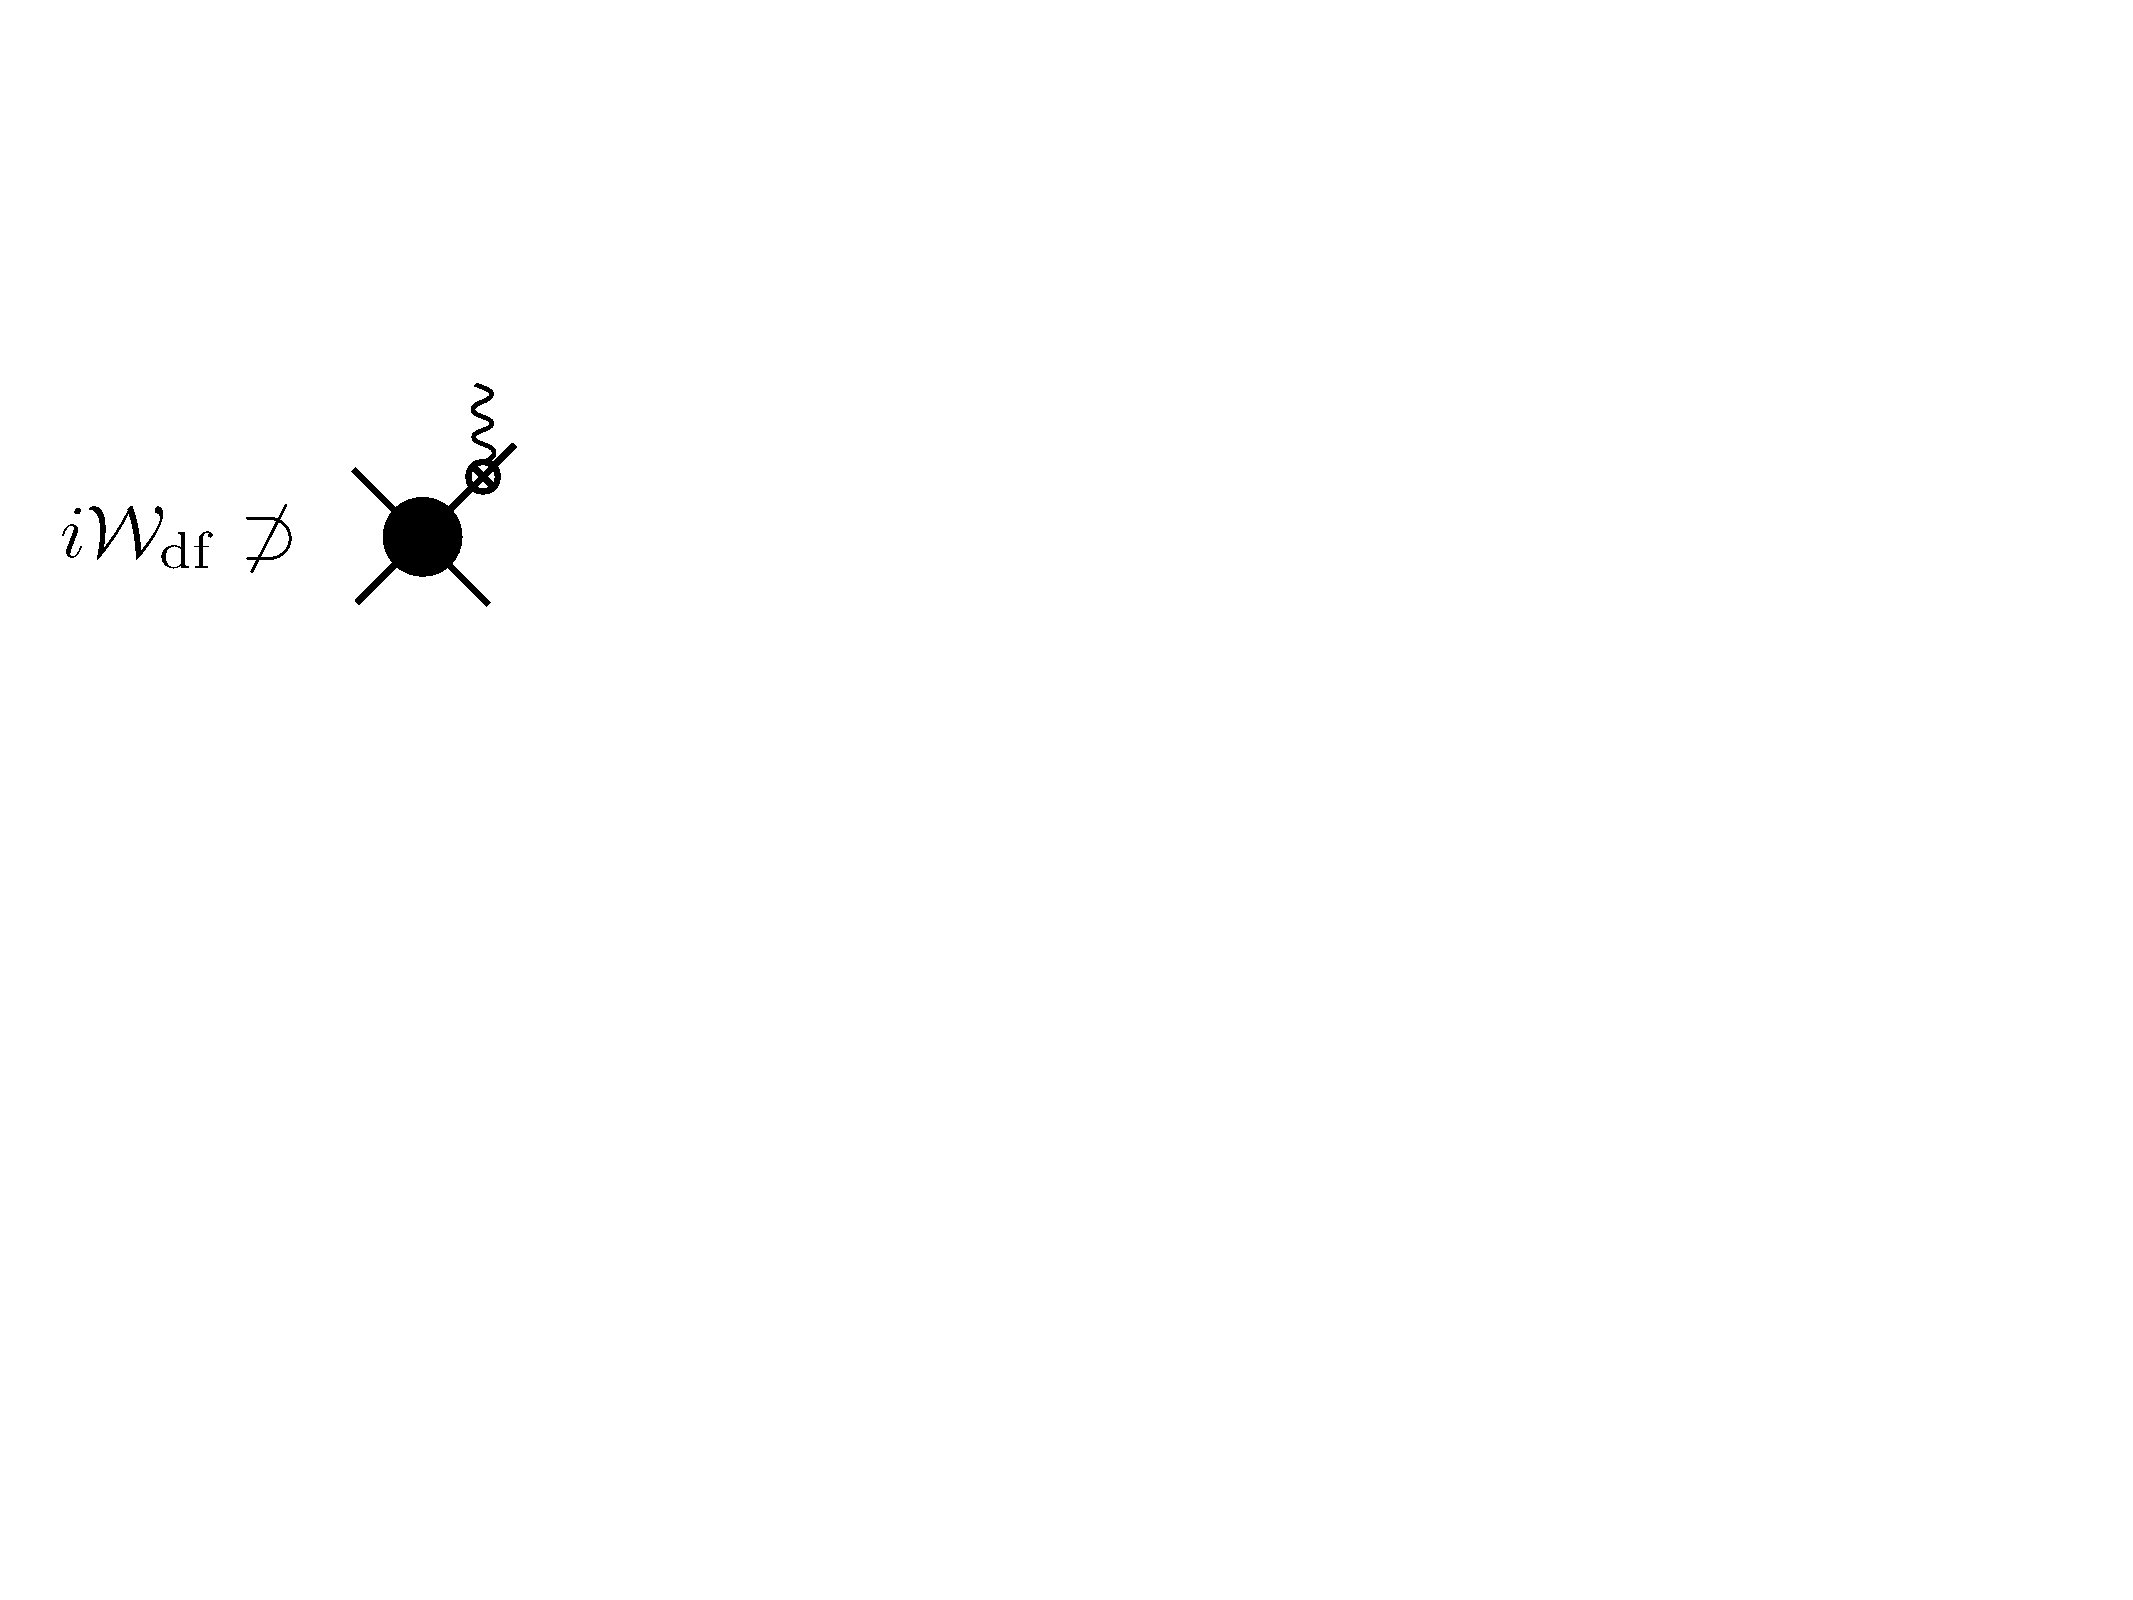
\includegraphics[scale=0.5]{figs/not_in_iWdf}}
\hspace{.5cm}
\subfigure[]{
\label{fig:IWdf_res_pole}
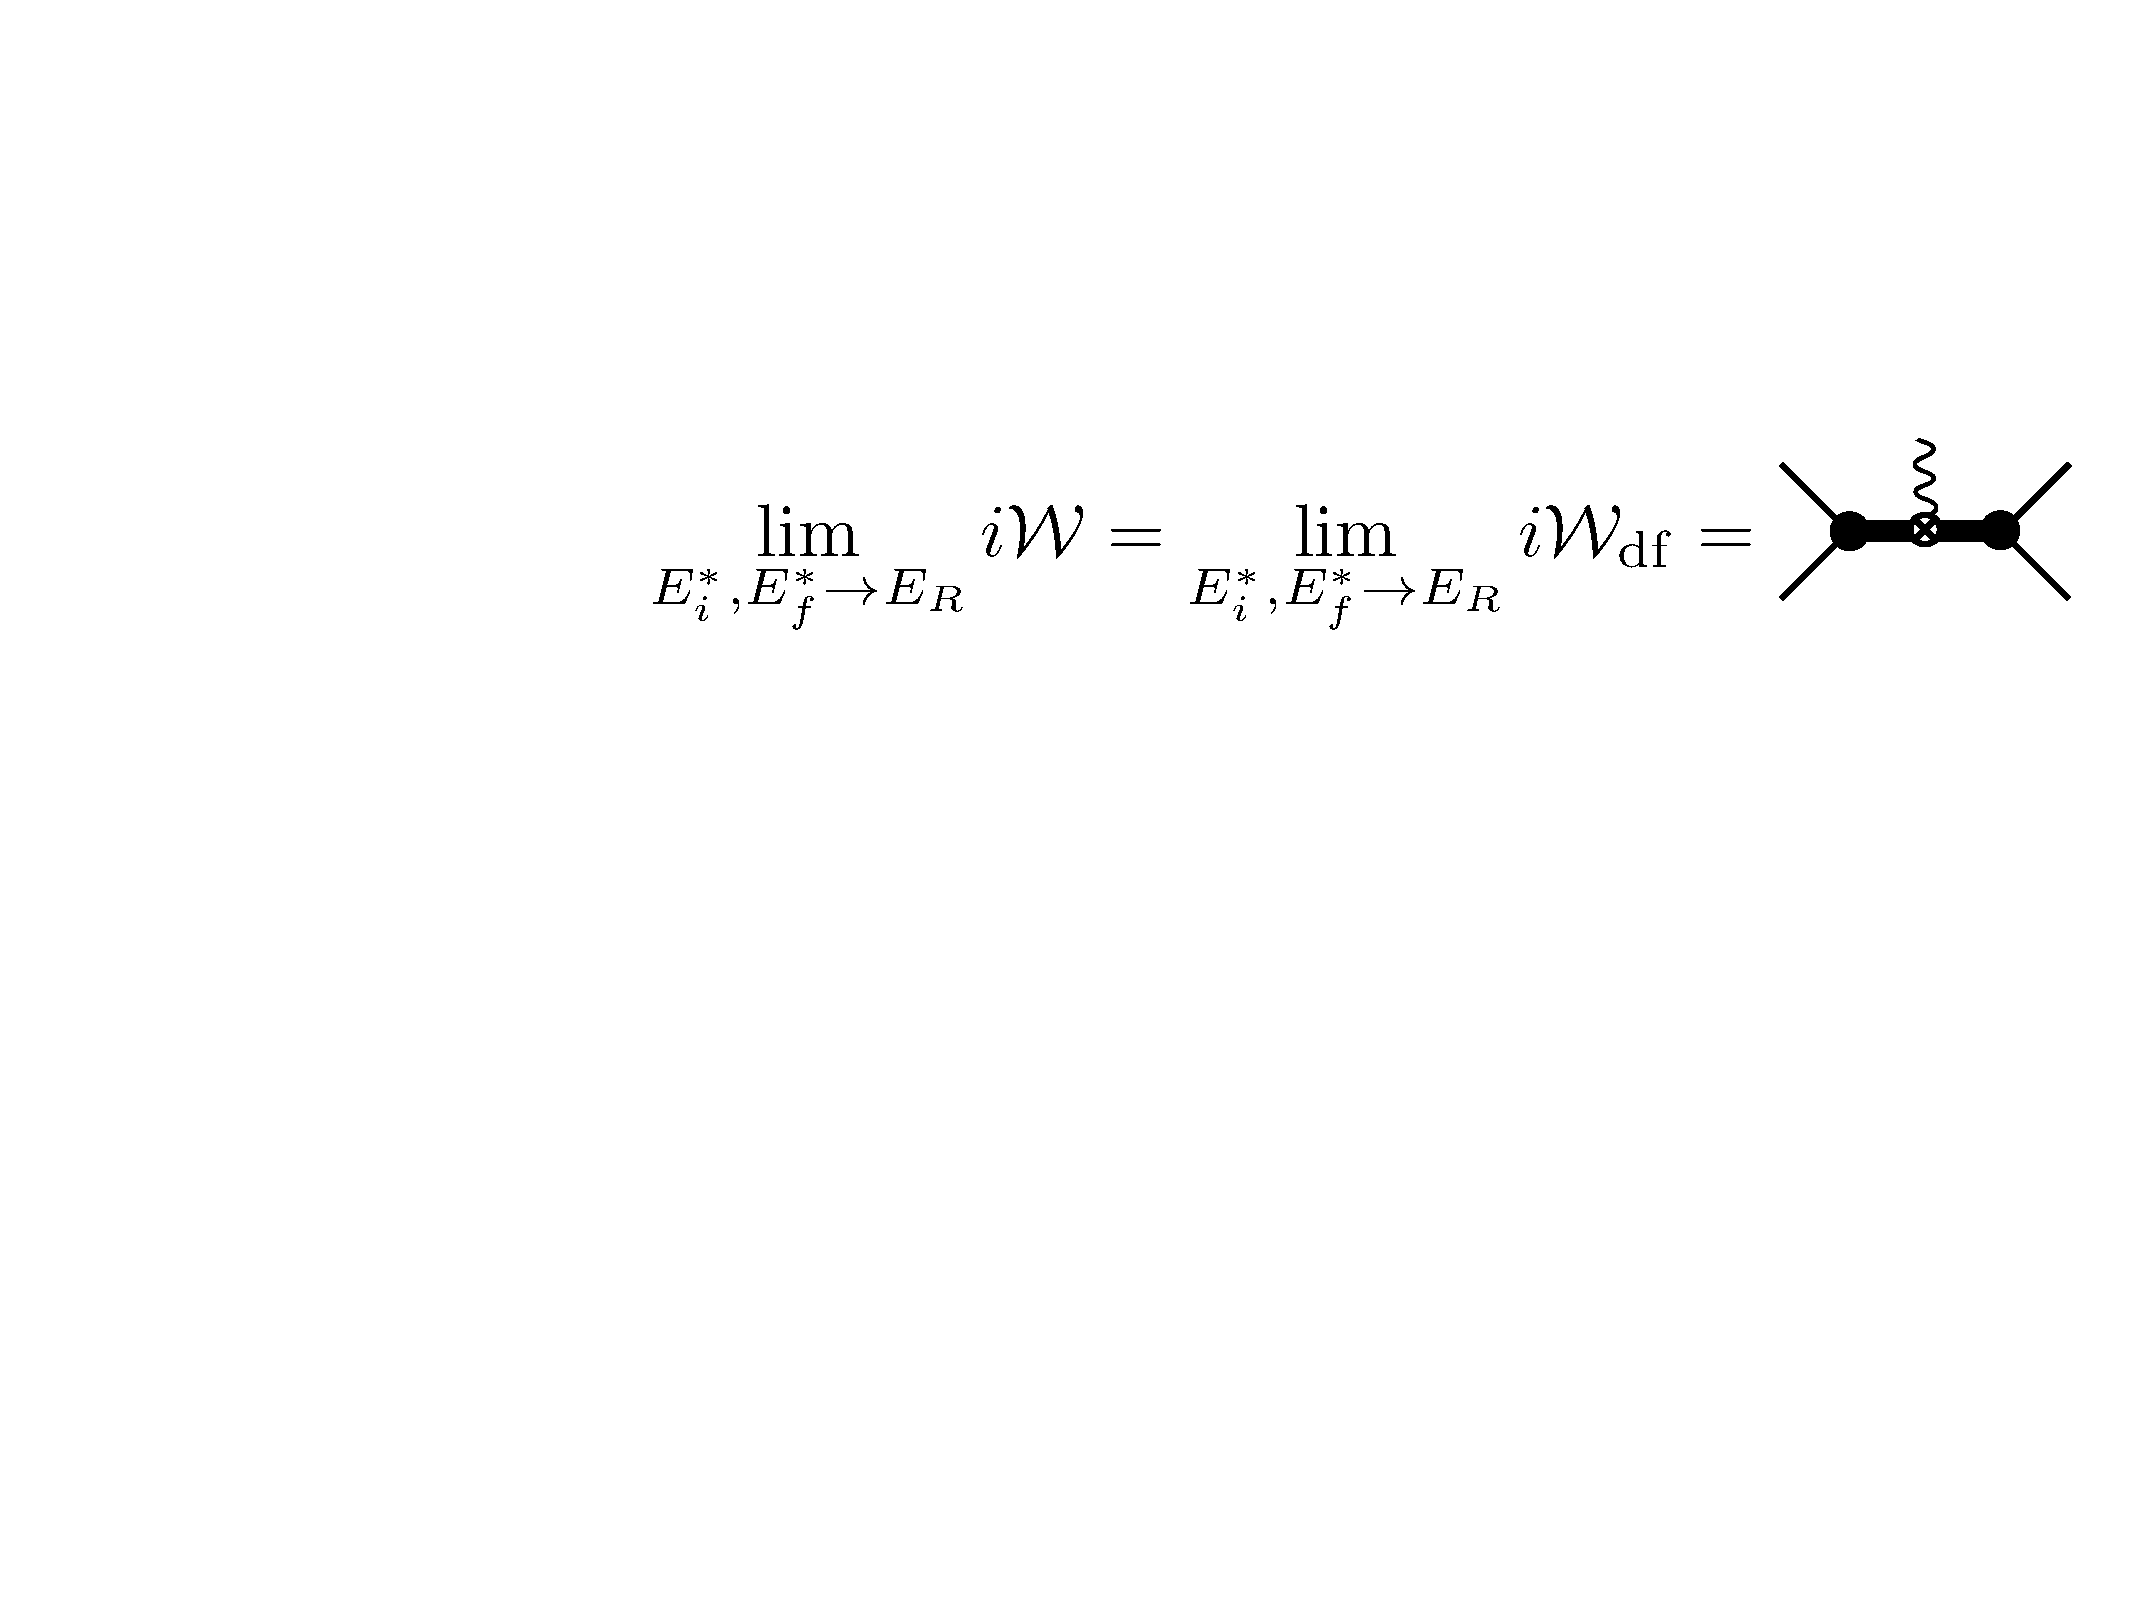
\includegraphics[scale=0.5]{figs/IWdf_res_pole}}
\caption{(a) Shown is an example of diagrams absent in $\Wdf$. (b) Shown is the postulate behavior of the $\Wdf$ near the resonance pole. }\label{fig:Wdf_pole}
\end{center}
\end{figure*}
%




\clearpage

